
% \title{Einbeziehen von \textsl{A-Priori}-Wissen, \glqq scharfer\grqq ~Model-Prior}
% \author{Dr.-Ing. Gerd Ehret, Dr. habil Dorothee Hüser \\ Physikalisch-Technische Bundesanstalt}
% \date{7. Jan. 2019}

% \title{\Large Parameterschätzung und Messunsicherheit mit der Bayesschen Statistik \\[2ex]}
% \author{Dozent: Dr.-Ing. Gerd Ehret \\ Physikalisch-Technische Bundesanstalt}
% date wird automatisch generiert
% \date{23. Oktober 2017} 
% Kommentierung uer mehrere Zeilen \begin{comment} \end{comment}
% \begin{document}
% \maketitle
% \begin{centering}
% 	\Large{Zehnte Vorlesung (Teil 1/2) zu} \\[1ex] 
%	\Large{\textbf{Messdatenauswertung und Messunsicherheit (MDA)}} \\[2ex]
%	\large{Modulverantwortlicher:} \\
%	\large{Prof. Dr.-Ing. R. Tutsch, iprom, TU Braunschweig}\\
% \end{centering}

\section{Einbeziehen von a-Priori-Wissen, \glqq scharfer\grqq ~Model-Prior}
\subsection{Kurze Wiederholung: Bayessche Statistik zur MU-Bestimmung}
In der 8. Vorlesung haben wir das Bayes-Theorem kennengelernt. 
Mit diesem ist es möglich a-Priori-Wissen $p(Y)$ über die zu bestimmende indirekte Messgröße $Y$ zu berücksichtigen.
Wir haben folgenden Zusammenhang kennengelernt: 
\begin{equation}
p(Y|X_1,\ldots,X_N) \propto l(Y|X_1,\ldots,X_N) \cdot p(Y) 
\label{eq:BayesTheorem}
\end{equation} 
bzw. 
\[
p(Y|X_1,\ldots,X_N) \propto p(X_1,\ldots,X_N|Y) \cdot p(Y) 
\] 
mit $p(Y)$ dem Prior der indirekten Messgröße $Y$ (auch oft als Ausgangsgröße bezeichnet), $l(Y|X_1,\ldots,X_N)$ Likelihood der Messdaten 
(Eingangsgrößen) $X_1,\ldots,X_N$. 

Die Likelihood kann auch -- wie in der 8. Vorlesung dargestellt -- als bedingte Wahrscheinlichkeitsdichte $p(X_1,\ldots,X_N|Y)$ aufgefasst werden. 

Der \textsl{Erwartungswert} $y := \operatorname{E}(Y)$ ist der \textsl{beste Schätzwert} für die Messgröße $Y$ und die \textsl{Varianz} ist ein 
\textsl{Maß für die Unsicherheit} $u^2(y) := \operatorname{Var}(Y)$.

\textbf{Beispiel: Bestimmung einer physikalischen Größe}\\
Wir betrachten ein Beispiel, bei dem irgendeine physikalische Größe zu messen ist.
Dabei werde ein Gerät bzw.\ Sensor verwendet, dessen Funktionsprinzip auf einem
physikalischen Effekt beruht und dadurch die Größe so erfasst,
dass als direkte Messgröße eine Spannung in Volt angezeigt wird. Dies kann beispielsweise
die Messung einer Temperatur sein, in der das Phänomen, dass sich ein elektrischer
Widerstand proportional zur Temperatur verändert und die Widerstandsänderung über die
Änderung der elektrischen Spannung, die über dem Widerstand abfällt, bestimmt wird.
Dies kann beispielsweise eine Stufenhöhe sein, die mit Hilfe eines induktiven Wegaufnehmers
gemessen wird, der auf dem Phänomen beruht, dass sich die Induktivität einer Spule in Abhängigkeit
von der  Position ihres Ferritkerns verändert. Es sind viele Beispiele denkbar. Sensoren
sind oft so konzipiert, dass sie ein physikalisches Phänomen nutzen und zur elektronischen
Erfassung der zu messenden Größe als direkte Größe ein Messignal in Form einer elektrischen
Spannung liefern.

Wir wollen im folgenden ganz allgemein die indirekte Messgröße mit $Y$
bezeichnen und uns auf keine physikalische Einheit festlegen, sondern diese allgemein nur
\glqq Einheit\grqq ~nennen. Das Modell, das wir betrachten, ist wie folgt: Das rohe Messsignal (Rohdaten),
das als Spannung $U$ bzw.\ direkte Größe $X_\mathrm{M}$ vorliegt, ist über
einen Kalibrierfaktor $K$ bzw.\ eine direkte Größe $X_\mathrm{K}$
in die indirekte physikalische Größe $Y$ umzurechnen. 
Der Index M steht hier für Messung und der Index K für Kalibrierfaktor.

In dem betrachteten Beispiel
ergebe das Produkt
\begin{equation}
Y \; = \; f(X_\mathrm{K}, X_\mathrm{M})  \; = \; X_\mathrm{K} \, X_\mathrm{M}
\end{equation}
der beiden direkten Größen $X_\mathrm{K}$ und $X_\mathrm{M}$ die indirekte Größe $Y$.

Um den Unterschied zwischen der bayesischen Statistik im eigentlichen Sinne
und einem Ansatz, der dem GUM Supplement 1 \cite{GUMS1} zugrunde gelegt wird, zu veranschaulichen,
werden wir uns klar machen, dass es einerseits die Sichtweise gibt,
\begin{itemize}
\item dass nicht nur die beiden direkten Messgrößen $X_\mathrm{K}$ und $X_\mathrm{M}$
Zufallsgrößen sind, sondern auch die indirekte Messgröße eine Zufallsgröße $Y$ ist
(\textbf{bayesische Statistik}),
die ihrerseits zusätzlich zu der Streuung der beiden direkten Größen einen Beitrag zur
Streuung liefert,
\end{itemize}
und andererseits,
\begin{itemize}
\item dass die Streuung der indirekten Größe $Y$ von der Streuung der beiden
direkten Messgrößen $X_\mathrm{K}$ und $X_\mathrm{M}$ herrührt, dass aber $Y$ selber von sich
aus nicht streut, sondern dass es
einen \textbf{\glqq scharfen\grqq ~\textsl{Model-Prior}} gibt.
\end{itemize}
Mit dem Begriff \glqq scharf\grqq ~ist hier gemeint, dass $Y \; = \; f(X_\mathrm{K}, X_\mathrm{M})$ keine Streuung haben würde, wenn die beiden direkten Größen
$X_\mathrm{K}$ und $X_\mathrm{M}$ keine Streuung hätten.

Der Einfachheit halber nehmen wir an, dass die Streuung der beiden direkten Größen
normalverteilt sei, so dass für deren Wahrscheinlichkeitsdichteverteilungen,
\textsl{Probability Density Functions} - kurz \textbf{pdf}s, folgendes gelte:
Der Kalibrierfaktor sei nach Herstellung des Sensors bestimmt worden mit einem Wert
$K_0$ und einer Unsicherheit $U_\mathrm{K}$, zu der der Erweiterungsfaktor mit $k = 2$
angegeben sei, so dass wir die Standardabweichung $s_\mathrm{K} = \frac{1}{2} U_\mathrm{K}$.
\begin{equation}
p_\mathrm{K} \propto 
 e^{\T -\;\frac{1}{2} \left(\frac{ X_\mathrm{K} - K_0}{s_\mathrm{K}} \right)^2}
\label{PriorKalibrierfaktor}
\end{equation}
Diese Verteilung betrachten wir als Prior, der in Abb.~\ref{fig:Kalibrierfaktor} dargestellt ist.
\begin{figure}[!htp]
	\begin{center}
%		\includegraphics[width=100mm]{Bilder/Kalibrierfaktor.eps}
		\includegraphics[width=140mm]{10_vorlesung/media/Kalibrierfaktor.png}
		\caption{Wahrscheinlichkeitsdichteverteilung, Prior, des
		Kalibrierfaktors zur Umrechnung der Sensordaten, die die physikalische
		Dimension einer Spannung in der Einheit Volt hat, in die Dimension der
		indirekten Messgröße $Y$ in ihrer Einheit.}
		\label{fig:Kalibrierfaktor}
	\end{center}
\end{figure}
Ferner sagen wir, dass wir in unserem Beispiel eine Stichprobe mit $J = 11$ Messwerten
mit dem Sensor aufgenommen haben, $(X_{\mathrm{M},1}, \dots, X_{\mathrm{M},J})$.
Der zu messende Gegenstand mit Messgröße $Y$, deren physikalische Einheit wir hier
ganz allgemein einfach \textsl{Einheit} nennen, solle so streuen, dass die gemessenen
Spannungswerte $(X_{\mathrm{M},1}, \dots, X_{\mathrm{M},J})$ mit $\sigma = 12$ Volt streuen.
Wir machen uns dazu klar, dass die Streuung von $\sigma = 12~\mathrm{V}$ nicht die Eigenschaft
des Sensors ist, sondern aus der Eigenschaft des Messgegenstands kommt!

Als {\`a}-priori Wissen zu dem Sensor kennen wir für einen Fall (A.) die Unsicherheit des
Sensors unabhängig von dem aktuell vorliegenden Gegenstand der Messung. Die dazu
proportionale Standardabweichung $s_\mathrm{S}$ des Sensors mit Index S für Sensor sei
signifikant kleiner als die Streuung der Daten der Stichprobe.

Ferner untersuchen wir Auswerteverfahren ohne Kenntnis der Unsicherheit des Sensors, für die
die gemeinsame Unsicherheit von Sensor und der Größe $Y$ des Gegenstands der Messung verwendet
wird, um die Likelihood zu berechnen, also eine Standardabweichung $s_\mathrm{M}$, die sich aus
der empirischen Varianz der Stichprobe ergibt. Dazu verwenden wir die Wurzel aus der empirischen
Varianz. Dies nennen wir Fall (B.).

Wir betrachen nun folgende vier Ansätze zur Bestimmung einer Posterior:

\begin{itemize}
	\item[(A.)] Präziser Sensor, 
	der die Rohdaten in der physikalischen Einheit Volt ausgibt und sehr wenig streut
	(z.~B. $s_\mathrm{S} = 0.3~\mathrm{V}$). Die sensorintrinsische Standardabweichung
	$s_\mathrm{S}$ wird für die Likelihood der direkten Messgröße $X_\mathrm{M}$ verwendet.
\begin{equation}
p_\mathrm{L} \propto \prod\limits_{j=1}^J 
e^{\T -\;\frac{1}{2} \left(\frac{ X_\mathrm{M} - X_{\mathrm{M},j} }{s_\mathrm{S}} \right)^2}
\label{LikeliGenauerSensor}
\end{equation}
	\item[(B.)] Das intrinsische Streuverhalten des Sensors sei unbekannt und damit nicht
	trennbar von der Streuung der Größe $Y$. Eine gemeinsame Streuung $s_\mathrm{M}$, die signifikant
	größer ist als die intrinsische Sensorstreuung $s_\mathrm{S}$ wird für die Likelihood der
	Sensorspannung $X_\mathrm{M}$ verwendet.
\begin{equation}
p_\mathrm{L} \propto \prod\limits_{j=1}^J 
e^{\T \; -\frac{1}{2} \left(\frac{X_\mathrm{M} - X_{\mathrm{M},j}}{s_\mathrm{M}} \right)^2}
\label{LikeliGemischteStreuung}
\end{equation}
\end{itemize}
In Abb.~\ref{fig:Rohdaten} ist die Likelihood gemäß Gl.~(\ref{LikeliGenauerSensor})
mit schwarzer, durchgezogener Kurve dargestellt. Sie setzt sich zusammen aus einzelnen
schmalen Peaks, Gaußverteilungen, weil die Breite der Normalverteilungen mit
$s_\mathrm{S} = 0.3~\mathrm{V}$ wesentlich schmaler ist als der Abstand zwischen den
einzelnen Stichprobenelementen. Gl.~(\ref{LikeliGemischteStreuung}) mit der gemeinsamen, breiten
Streuung, die von der Streuung des Messgegenstandes dominiert wird, ist als rot gestrichelte
Kurve eingezeichnet. Hier sehen wir eine gemeinsame, breite Normalverteilung.

\begin{figure}[!htp]
	\begin{center}
%		\includegraphics[width=100mm]{Bilder/Rohdaten.eps}
		\includegraphics[width=120mm]{10_vorlesung/media/Rohdaten.png}
		\caption{Likelihood (Wahrscheinlichkeitsdichtefunktion pdf)
		der direkt gemessenen Größe $X_\mathrm{M}$, der Rohdaten: Schwarze, durchgezogene Linie
		für die pdf mit {\`a}-priori-Wissen über die Genauigkeit des Sensors/Messgerätes
		(\glqq Geraet genau\grqq);
		rote gestrichelte Kurve für die pdf für unbekannte Streuung vom Gerät,
		mit der aus der empirischen Standardabweichung der Rohdaten
		bestimmten Streuung, so dass das Gerät als ungenau erscheint erscheint (\glqq Geraet ungenau\grqq)}
		\label{fig:Rohdaten}
	\end{center}
\end{figure}
\newpage
\begin{enumerate}
	\item Im Fall 1 verwenden wir die Likelihood mit bekannter Streuung 
	$s_\mathrm{S} = 0.3~\mathrm{V}$ des Präzisions\-sensors (A.), Gl.~(\ref{LikeliGenauerSensor}),
	zusammen mit der Verteilung des Kalibrierfaktors, dem Prior Gl.~(\ref{PriorKalibrierfaktor}),
	und einer Normalverteilung für die indirekte Messgröße $Y$ mit einer zu
	schätzenden Standardabweichung $\sigma_Y$:
\begin{equation}
p_\mathrm{Modell} (X_\mathrm{K}, X_\mathrm{M} | Y, \sigma_Y) \propto
e^{\T -\;\frac{1}{2} \left(\frac{ Y \; - \; X_\mathrm{K} \, X_\mathrm{M}}{\sigma_Y} \right)^2}
\qquad \mathrm{mit} \qquad
(J-1) \left(\frac{\sigma_Y}{s_\mathrm{KM}}\right)^2 \sim \chi^2
\label{pdfModellNormalverteilt}
\end{equation}
	Dabei ist $s_\mathrm{KM}$ eine zur Streuung der Rohdaten proportionale Größe
	$s_\mathrm{KM} \; = \; K_0 \, s_\mathrm{M}$. Der Faktor $K_0$ ist der {\`a}-priori
	bekannte Schätzer des Kalibrierfaktors.
	Die Posterior ist dann
\begin{equation}
\arraycolsep=2.0pt\def\arraystretch{2.0}
\begin{array}{l}
p(Y, X_\mathrm{K}, X_\mathrm{M}, \sigma_Y | (X_{\mathrm{M},1}, \dots, X_{\mathrm{M},J}), K_0, s_\mathrm{K}, s_\mathrm{S}) \propto \\
e^{\T-\;\frac{1}{2} \left(\frac{ Y \; - \; X_\mathrm{K} \, X_\mathrm{M}}{\sigma_Y} \right)^2}
\; \prod\limits_{j=1}^J \,
e^{\T -\;\frac{1}{2} \left(\frac{ X_\mathrm{M} - X_{\mathrm{M},j} }{s_\mathrm{S}} \right)^2}
\;  e^{\T-\;\frac{1}{2} \left(\frac{X_\mathrm{K} - K_0}{s_\mathrm{K}} \right)^2}
\; p_{\chi^2} ((J-1) \left(\frac{\sigma_Y}{s_\mathrm{KM}}\right)^2) .
\end{array}
\label{PosteriorFall1}
\end{equation}
	\item Im Fall 2 betrachten wir für die Likelihood (B.) der direkten Messgröße $X_\mathrm{M}$
	die Standardabweichung $s_\mathrm{M}$, Gl.~(\ref{LikeliGemischteStreuung}), und für 
	Verteilung B (\glqq Gerät ungenau\grqq) ~in Kombination mit der Verteilung des
	Kalibrierfaktors und für die
	Modellverteilung nehmen wir wieder eine Standardabweichung $s_\mathrm{KM}$ 
	an.
\begin{equation}
\arraycolsep=2.0pt\def\arraystretch{2.0}
\begin{array}{l}
p(Y, X_\mathrm{K}, X_\mathrm{M}, \sigma_Y | (X_{\mathrm{M},1}, \dots, X_{\mathrm{M},J}), K_0, s_\mathrm{K}) \propto \\
e^{\T-\;\frac{1}{2} \left(\frac{ Y \; - \; X_\mathrm{K} \, X_\mathrm{M}}{\sigma_Y} \right)^2}
\; \prod\limits_{j=1}^J \,
e^{\T-\;\frac{1}{2} \left(\frac{ X_\mathrm{M} - X_{\mathrm{M},j} }{s_\mathrm{M}} \right)^2}
\;  e^{\T-\;\frac{1}{2} \left(\frac{X_\mathrm{K} - K_0}{s_\mathrm{K}} \right)^2}
\; p_{\chi^2} ((J-1) \left(\frac{\sigma_Y}{s_\mathrm{KM}}\right)^2)
\end{array}
\label{PosteriorFall2}
\end{equation}
	mit $s_\mathrm{M}$ für die empirische Standardabweichung berechnet aus der Stichprobe
	$(X_{\mathrm{M},1},$ $\dots,$ $X_{\mathrm{M},J})$.
	\item Im Fall 3 nehmen wir genauso wie in Fall 2 wieder (B.) (\glqq Gerät ungenau\grqq)
	dieselbe Likelihood
	und verwenden wie gehabt die Verteilung des Kalibrierfaktors. Wir wollen jetzt den Übergang zu dem
	Ansatz mit scharfem \textsl{Model-Prior} bekommen, indem wir für $\sigma_Y$ einen sehr, sehr
	kleinen Wert einsetzen, so dass die Verteilungsdichte für das Modell
	Gl.~(\ref{pdfModellNormalverteilt}) sehr schmal wird, weil die Dirac-Funktion als
	Normalverteilung für $\sigma \rightarrow 0$ interpretiert werden kann.
\begin{equation}
\arraycolsep=2.0pt\def\arraystretch{2.0}
\begin{array}{l}
p(Y, X_\mathrm{K}, X_\mathrm{M} | (X_{\mathrm{M},1}, \dots, X_{\mathrm{M},J}), K_0, s_\mathrm{K}) \propto \\
e^{\T-\;\frac{1}{2} \left(\frac{ Y \; - \; X_\mathrm{K} \, X_\mathrm{M}}{\sigma_\mathrm{winzig}} \right)^2}
\; \prod\limits_{j=1}^J  \,
e^{\T-\;\frac{1}{2} \left(\frac{ X_\mathrm{M} - X_{\mathrm{M},j} }{s_\mathrm{M}} \right)^2}
\;  e^{\T-\;\frac{1}{2} \left(\frac{X_\mathrm{K} - K_0}{s_\mathrm{K}} \right)^2}
\end{array}
\label{PosteriorFall3}
\end{equation}
	mit $\sigma_\mathrm{winzig} \; = \; 0.003 \cdot s_\mathrm{KM}$.
	\item Im Fall 4 wird für die pdf des Modells der Grenzübergang
	$\sigma_Y \rightarrow 0$ vollzogen, siehe Paper von Wuebbler et al. 
	\cite{Wue08}, also
\begin{equation}
p_\mathrm{Modell} (X_\mathrm{K}, X_\mathrm{M} | Y) \propto
\lim\limits_{\sigma_Y \rightarrow 0} \, \frac{1}{\sigma_Y} \,
e^{\T-\;\frac{1}{2} \left(\frac{ Y \; - \; X_\mathrm{K} \, X_\mathrm{M}}{\sigma_Y} \right)^2} \; = \;
\delta(Y \; - \; X_\mathrm{K} \, X_\mathrm{M})
\label{pdfModellDiracPeak}
\end{equation}
oder allgemein für jedes Modell der Gestalt $Y \; = \; f(X_1, \dots X_N)$
\begin{equation}
p_\mathrm{Modell} (X_\mathrm{K}, X_\mathrm{M} | Y) \propto
\lim\limits_{\sigma_Y \rightarrow 0}  \, \frac{1}{\sigma_Y} \,
e^{\T-\;\frac{1}{2} \left(\frac{ Y \; - \; f(X_1, \dots X_N)}{\sigma_Y} \right)^2} \; = \;
\delta(Y \; - \; f(X_1, \dots X_N) ) .
\label{pdfallgemeinesModellDiracPeak}
\end{equation}
	Damit sieht der Posterior wie folgt aus
\begin{equation}
\arraycolsep=2.0pt\def\arraystretch{2.0}
\begin{array}{l}
p(Y, X_\mathrm{K}, X_\mathrm{M} | (X_{\mathrm{M},1}, \dots, X_{\mathrm{M},J}), K_0, s_\mathrm{K}) \propto \\
\delta \left( Y \; - \; X_\mathrm{K} \, X_\mathrm{M}\right)
\; e^{\T-\;\frac{1}{2} \left(\frac{ X_\mathrm{M} - X_{\mathrm{M},j} }{s_\mathrm{M}} \right)^2}
\;  e^{\T-\;\frac{1}{2} \left(\frac{X_\mathrm{K} - K_0}{s_\mathrm{K}} \right)^2}.
\end{array}
\label{PosteriorFall4}
\end{equation}
\end{enumerate}

Wir berechnen für die jeweiligen Posteriors wieder die jeweilige
Marginalverteilung, bei der die Posterior als
Funktion von $Y$ gewonnen wird, indem über die Größen $X_\mathrm{K}$, $X_\mathrm{M}$
und $\sigma_Y$ integriert wird. Bei dem im Anhang abgedruckten Matlab/Gnu-Octaveskript wurde
eine Vereinfachung vorgenommen, indem darauf verzichtet wurde, für $\sigma_Y$ eine
Verteilungsdichtefunktion $p_{\chi^2} ((J-1) \left(\frac{\sigma_Y}{s_\mathrm{KM}}\right)^2)$ zu
verwenden und dann über $\sigma_Y$ zu integrieren. Hier wurde einfach nur für $\sigma_Y$
die zur Streuung der Rohdaten proportionale Streuung $s_\mathrm{KM}$ eingesetzt, also
$\sigma_Y = s_\mathrm{KM}$. Um von der Überdeckung her sicherer zu sein, haben wir diese aufgrund des
sehr kleinen Stichprobenumfangs noch mit einem heuristischen Faktor $c > 1$ multipliziert
$$
s_\mathrm{KM} \; = \; c \, K_0 \, s_\mathrm{M} ,
$$
so dass für die Posteriors der Fälle 1 und 2 folgende Integrationen durchgeführt wurden
\begin{equation}
\arraycolsep=2.0pt\def\arraystretch{2.0}
\begin{array}{l}
p(Y | (X_{\mathrm{M},1}, \dots, X_{\mathrm{M},J}), K_0, s_\mathrm{K}, s_\mathrm{S}) \propto \\
\int\limits_{-\infty}^\infty \int\limits_{-\infty}^\infty \,
e^{\T-\;\frac{1}{2} \left(\frac{ Y \; - \; X_\mathrm{K} \, X_\mathrm{M}}{\sigma_Y} \right)^2}
\; \prod\limits_{j=1}^J  \,
e^{\T-\;\frac{1}{2} \left(\frac{ X_\mathrm{M} - X_{\mathrm{M},j} }{s_\mathrm{S}} \right)^2}
\;  e^{\T-\;\frac{1}{2} \left(\frac{X_\mathrm{K} - K_0}{s_\mathrm{K}} \right)^2}  \,
\operatorname{d}X_\mathrm{M} \, \operatorname{d}X_\mathrm{K}
\end{array}
\label{marginalPosteriorFall1}
\end{equation}
für Fall 1, bei dem $s_\mathrm{S}$ die aus vorheriger Charakterisierung des
Sensors, d.h.\ aus {\`a}-priori Wissen, bekannte Standardabweichung der Sensorspannung ist
und 
\begin{equation}
\arraycolsep=2.0pt\def\arraystretch{2.0}
\begin{array}{l}
p(Y | (X_{\mathrm{M},1}, \dots, X_{\mathrm{M},J}), K_0, s_\mathrm{K}) \propto \\
\int\limits_{-\infty}^\infty \int\limits_{-\infty}^\infty \,
e^{\T-\;\frac{1}{2} \left(\frac{ Y \; - \; X_\mathrm{K} \, X_\mathrm{M}}{\sigma_Y} \right)^2}
\;\prod\limits_{j=1}^J \,
 e^{\T-\;\frac{1}{2} \left(\frac{ X_\mathrm{M} - X_{\mathrm{M},j} }{s_\mathrm{M}} \right)^2}
\;  e^{\T-\;\frac{1}{2} \left(\frac{X_\mathrm{K} - K_0}{s_\mathrm{K}} \right)^2} \,
\operatorname{d}X_\mathrm{M} \, \operatorname{d}X_\mathrm{K}
\end{array}
\label{marginalPosteriorFall2}
\end{equation}
für Fall 2, bei dem $s_\mathrm{M}$ die aus der Stichprobe
$(X_{\mathrm{M},1}, \dots, X_{\mathrm{M},J})$ berechnete empirische
Standardabweichung ist.

Die Marginalverteilung zu Posterior Gl.~(\ref{PosteriorFall4}) für Fall 4, also
die pdf als Funktion von $Y$, sieht wie folgt aus
\begin{equation}
\arraycolsep=2.0pt\def\arraystretch{2.0}
\begin{array}{l}
p(Y | (X_{\mathrm{M},1}, \dots, X_{\mathrm{M},J}), K_0, s_\mathrm{K}) \propto \\
\int\limits_{-\infty}^\infty \int\limits_{-\infty}^\infty \,
\delta \left( Y \; - \; X_\mathrm{K} \, X_\mathrm{M}\right)
\; \prod\limits_{j=1}^J  \,
e^{-\frac{1}{2} \left(\frac{ X_\mathrm{M} - X_{\mathrm{M},j} }{s_\mathrm{M}} \right)^2}
\;  e^{-\frac{1}{2} \left(\frac{X_\mathrm{K} - K_0}{s_\mathrm{K}} \right)^2}  \,
\operatorname{d}X_\mathrm{M} \, \operatorname{d}X_\mathrm{K}.
\end{array}
\label{marginalPosteriorFall4}
\end{equation}
Damit berechnen wir für alle möglichen Paare $X_\mathrm{K}, X_\mathrm{M}$ direkt je ein
$Y$ mit $Y = X_\mathrm{K} \, X_\mathrm{M}$. Zu jedem der Paare $X_\mathrm{K}, X_\mathrm{M}$
berechnen wir die Wahrscheinlichkeit
$$
p(X_\mathrm{K} \, X_\mathrm{M}) \propto \prod\limits_{j=1}^J  \,
e^{-\frac{1}{2} \left(\frac{ X_\mathrm{M} - X_{\mathrm{M},j} }{s_\mathrm{M}} \right)^2}
\;  e^{-\frac{1}{2} \left(\frac{X_\mathrm{K} - K_0}{s_\mathrm{K}} \right)^2},
$$
die dann die pdf als Funktion von $Y$ ist.

In dem im Anhang gezeigten Matlab/Gnu-octaveskript haben wir für die Größen
$X_\mathrm{K}$ und $X_\mathrm{M}$ ein äquidistant gerastertes Gitter verwendet und alle
Möglichkeiten durchgerechnet. Das lässt sich bei diesem kleinen Beispiel und der Leistung
der heutigen Rechentechnik leicht durchführen. Bei umfangreicheren Problemstellungen jedoch
ist diese \glqq brute force\grqq ~nicht sinnvoll. Für solche Fälle
werden solche Samples für die direkten Messgrößen
gewählt, die bereits berücksichtigen, wie ihre Wahrscheinlichkeitsdichteverteilungen aussehen.
Dies können nichtäquidistante, deterministische Samples sein, deren Intervalle enger sind
je größer die Wahrscheinlichkeit ist. Dies können aber auch stochastisch gewählte Samples sein,
die sich ebenfalls an der Wahrscheinlichkeitsdichte der direkten Größen orientieren.
Für die stochastischen Samples werden Pseudozufallszahlen eingesetzt, also Zahlen, die zufällig
aussehen, die aber mit deterministischen, numerischen Algorithmen berechnet werden.
Wegen des zufälligen Charakters der Zahlen, den auch Zahlen, die bei Spielen mit Würfeln und
Roulettescheiben gefunden werden, haben, werden diese Methoden \textbf{Monte-Carlo-Methoden}
genannt.


Abb.~\ref{fig:Posteriorverteilungen_4Faelle} zeigt alle vier Posteriormarginalverteilungen,
die pdf für Fall 1 gemäß Gl.~(\ref{marginalPosteriorFall1}) als schwarze, durchgezogene Linie mit
der Bezeichung in der Legende \glqq Geraet genau, Messobjekt schlecht\grqq, die pdf für
Fall 2 gemäß Gl.~(\ref{marginalPosteriorFall2}) als rote, gestrichelte Linie mit der
Bezeichnung \glqq beides ungenau\grqq, die Marginalverteilung
zu Gl.~(\ref{PosteriorFall3}) als blaue, durchgezogene Kurve und die
Wahrscheinlichkeiten zu den paarweise berechneten Werten für $Y$ gemäß der Marginalverteilung
mit dem scharfen \textsl{Model-Prior} Gl.~(\ref{marginalPosteriorFall4}).
\begin{figure}[!htb]
	\begin{center}
%		\includegraphics[width=100mm]{Bilder/posterior.eps}
		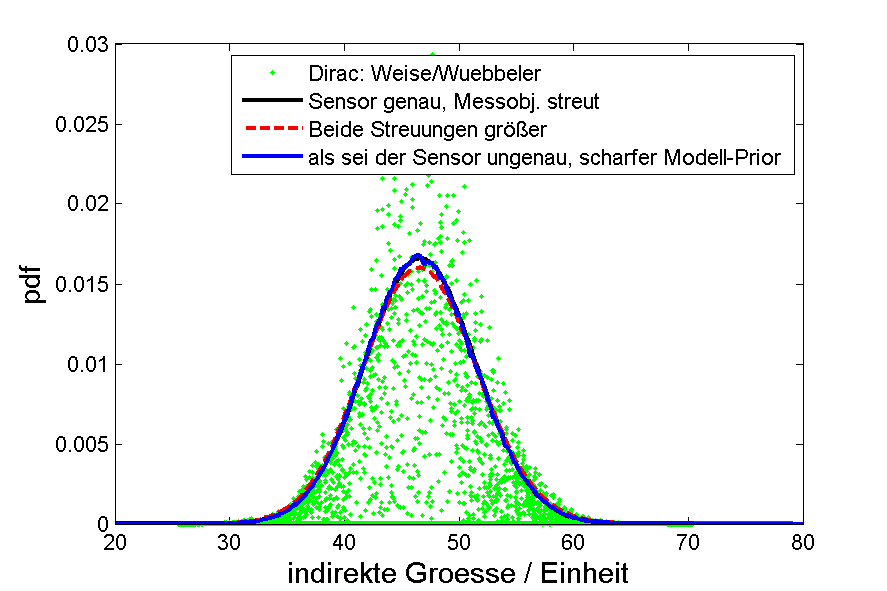
\includegraphics[width=130mm]{10_vorlesung/media/Posterior_all.png}
		\caption{Posteriorverteilungen für die Bestimmung der
			indirekten Größe für die 4 Fälle}
		\label{fig:Posteriorverteilungen_4Faelle}
	\end{center}
\end{figure}

\newpage

\subsection{Modellgleichung als {\`a}-Priori-Wissen $\rightarrow$  klass. Statistik}

Wenn eine Modellgleichung gegeben ist, so kann diese als {\`a}-Priori-Wissen miteinbezogen werden. 
Gegeben sei die Modellgleichung zwischen der gesuchten 
Messgröße $Y$ und den direkten Messgröße $X_1,\ldots, X_N$, die wir auch in einem
Vektor $\boldsymbol{X} := (X_1 \ldots  X_N)$ schreiben
\begin{equation}
Y = f(X_1,\ldots,X_N) = f(\boldsymbol{X})
\label{eq:Modellgleichung}
\end{equation}
Werden alle Größen, sowohl die direkten $\boldsymbol{X} := (X_1 \ldots  X_N)$ als
auch die indirekte Größe $Y$ als Zufallsgrößen angesehen, so gibt es zu jeder der
Größen eine stochastische Komponente, die wir oftmals als normalverteilt erachten können.
Wir können aber auch für bestimmte physikalische Gegebenheiten, wie beispielsweise Störungen
durch Vibrationen, als verteilt nach einem Arcussinus-Verhalten berechnen.
Zu jeder der Größen gibt es also Abweichungen, so dass wir schreiben
\begin{equation}
Y + \varepsilon_\mathrm{Y-all} = f(X_1 + \varepsilon_1,\ldots,X_N + \varepsilon_N) + \varepsilon_\mathrm{Y-intrinsisch}
\label{eq:ModellgleichungAlleZufall}
\end{equation}
Wir wollen im weiteren Fall 4 des oben dargelegten Beispiels, nämlich den Fall eines
\textbf{scharfen Model-Priors}, genauer beleuchten. Mit dem Begriff des scharfen
Model-Priors ist gemeint, dass das Modell
selber scharf ist, also Gl.~(\ref{eq:Modellgleichung}) genau so gilt und nur die direkten
Größen als Zufallsgrößen erachtet werden
\begin{equation}
Y + \varepsilon_\mathrm{Y} = f(X_1 + \varepsilon_1,\ldots,X_N + \varepsilon_N)
\label{eq:ModellgleichungDirekteZufall}
\end{equation}
sodass die Abweichungen $\varepsilon_\mathrm{Y}$ der indirekten Größe $Y$ allein von
den Abweichungen $\varepsilon_i$ der direkten Größen abhängt und keine der Größe
$Y$ eigene (intrinsische) Abweichung zugeordnet wird.
\begin{equation}
\varepsilon_\mathrm{Y} \; \approx \;
\sum\limits_{i=1}^N \frac{\partial}{\partial X_i} f(X_1 + \varepsilon_1,\ldots,X_N + \varepsilon_N)
\, \varepsilon_i \; + \; \mathcal{O}(\varepsilon_i^2)
\label{eq:epsilonY}
\end{equation}
Das heißt es gelte der in Gl.~(\ref{pdfallgemeinesModellDiracPeak}) vorgenommene
Grenzübergang, der auch dem entspricht, dass wir sagen
$$
\varepsilon_\mathrm{Y-intrinsisch} \rightarrow 0
$$
und es wird für die indirekte Messgröße keine Verteilung mehr angenommen.
Anders ausgedrückt heißt es, dass bei einem gemessenen Satz an Eingangsgrößen,
sich die Ausgangsgröße nach der Modellgleichung Gl.(\ref{eq:Modellgleichung}) berechnet,
so wird die gesuchte Messgröße $Y$ festgelegt. Man kann sich das auch so vorstellen, dass
die angenommene Modellverteilung immer schmaler wird und somit nur 
noch ein $Y_j$ Wert bei jeder Beobachtung $\boldsymbol{X}_j = (X_{1,j}, \dots X_{N,j})$ 
erlaubt ist.
Diesen Übergang stellt auch Abb. \ref*{fig:Uebergang_Delta_Funktion} dar. 
\begin{figure}[!htp]
	\begin{center}
		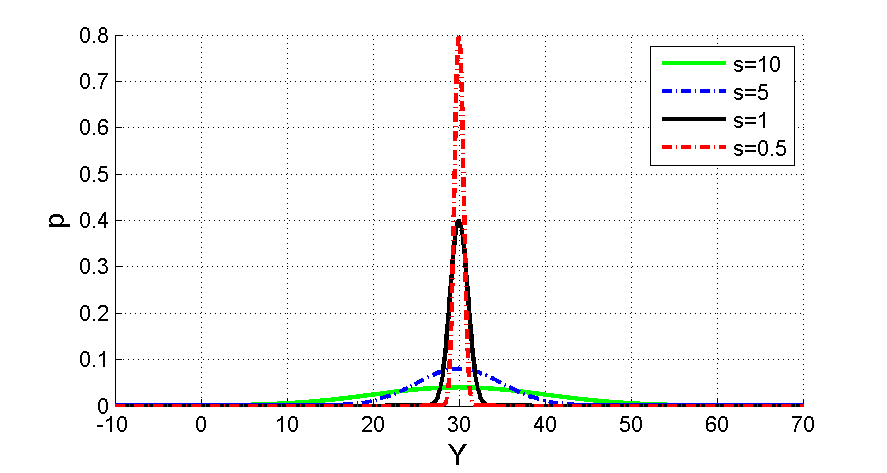
\includegraphics[width=130mm]{10_vorlesung/media/DeltaPeaken.png}
		\caption{Übergang von Bayes-Statistik zur klassischen Statistik mit immer schmaler werdenden angenommenen Verteilungen für $Y$}
		\label{fig:Uebergang_Delta_Funktion}
	\end{center}
\end{figure}

Wir verwenden
gemäß Gl.~(\ref{pdfallgemeinesModellDiracPeak}) den \textbf{Model-Prior} als Dirac'sche delta-Funktion: 
\begin{equation}
\delta(Y-f(\boldsymbol{X}))
\end{equation}
Dadurch, dass wir hier $Y$ festlegen sind wir nicht mehr in der 
Bayes-Welt (Bayes-Statistik), sondern wieder in der klassischen 
Statistik. 
Durch Messungen oder andere Informationen seien 
\textbf{Wahrscheinlichkeitsdichteverteilungen der Messdaten} $\boldsymbol{X}$
gegeben, d.h.
\begin{equation}
p(\boldsymbol{X})
\end{equation}
Darüberhinaus können haben wir zusätzliche Informationen über die Größe
$Y$ in die statistische Analyse einarbeiten, beispielsweise Ergebnisse
aus anderen Instituten oder aus vergangenen Messkampagnen. 
Die können wir ganz genau so behandeln wie den Prior in der
bayes'schen Statistik. Da wir von den anderen Instituten oder Messkampagnen
keine direkten Größen und somit auch keine Likelihood vorliegen haben, verwenden
wird eine Wahrscheinlichkeitsdichteverteilung für $Y$ gemäß den Annahmen über
die Streuung von $Y$, die aus dem vollständigen Messergebnis des anderen Instituts oder
der anderen Messkampagne hervorgeht. Dies kann eine Normalverteilung, eine Student-t-Verteilung
oder dergleichen sein. Die Wahrscheinlichkeitsdichteverteilung (PDF) des
Priors zu $Y$ kennzeichnen wir hier mit einem Index 
\glqq Null\grqq, also $p_0(Y)$ (\textbf{Prior der Messgröße} $Y$) 
\begin{equation}
p_0(Y)
\end{equation}
Wir können nun eine gemeinsame PDF für $\boldsymbol{Z} = (\boldsymbol{X},Y)$
aufstellen, die wie folgt gegeben ist \cite{Els07}: 
\begin{equation}
p(\boldsymbol{Z}) = p(\boldsymbol{X},Y) \propto p(\boldsymbol{X}) \cdot p_0(Y) \cdot \delta(Y-f(\boldsymbol{X})) 
\end{equation}
Die gesuchte PDF für die Messgröße $Y$ erhalten wir durch Marginalisierung der $p(\boldsymbol{X},Y)$ über $X$:
\begin{equation}
p(Y) = \int_{-\infty}^{\infty} p(\boldsymbol{X'},Y) \mathrm{d} X'
\propto p_0(Y)\int_{-\infty}^{\infty}  p(\boldsymbol{X'}) \cdot \delta(Y-f(\boldsymbol{X'})) \mathrm{d} \boldsymbol{X'} 
\label{eq:pdf_Y_durch_Marginalisierung}
\end{equation}
Den besten Schätzwert für $Y$ erhalten wir wieder über den 
Erwartungswert $y=E(Y)$:
%\begin{equation}
\begin{align}
y &= \int Y' p(Y') dY' \nonumber\\ 
&=  \int Y'\frac{\T p_0(Y) \int p(\boldsymbol{X'}) \cdot \delta(Y'-f(\boldsymbol{X}')) \mathrm{d} \boldsymbol{X}' }
{\T \int p_0(Y'')\int  p(\boldsymbol{X}') \cdot \delta(Y''-f(\boldsymbol{X}')) \mathrm{d} \boldsymbol{X}'\mathrm{d} \boldsymbol{Y}'' } \mathrm{d} Y'  \nonumber \\[2ex]
&= \frac{\T\int \left( \int Y' \cdot p_0(Y) \cdot p(\boldsymbol{X}') \cdot \delta(Y'-f(\boldsymbol{X}'))\mathrm{d}Y' \right) \mathrm{d} \boldsymbol{X}' }
{\T \int \left(\int p_0(Y'') p(\boldsymbol{X}') \cdot \delta(Y''-f(\boldsymbol{X}')) \mathrm{d}  \boldsymbol{Y}'' \right) \mathrm{d} \boldsymbol{X}'}\nonumber \\[2ex]  
&=  \frac{\T\int f(\boldsymbol{X}') \cdot p_0(f(\boldsymbol{X}')) \cdot p(\boldsymbol{X}')  \mathrm{d} \boldsymbol{X}' }
{\T \int   p_0(f(\boldsymbol{X}')) \cdot p(\boldsymbol{X}') 
	\mathrm{d} \boldsymbol{X}'}  \label{eq:schaetzwert_y}
\end{align}
% \end{equation}
Die Unsicherheit ergibt sich aus der Varianz von $Y$  
\begin{align}
u^2(y) &= \int (y-Y')^2 p(Y') dY' \nonumber \\[2ex]
&= \frac{\T \int (y-f(\boldsymbol{X}'))^2 \cdot p_0(f(\boldsymbol{X}'))
	\cdot p(\boldsymbol{X}') \mathrm{d} \boldsymbol{X}' }
{\T p_0(f(\boldsymbol{X}')) \cdot p(\boldsymbol{X}') \mathrm{d} \boldsymbol{X}'}  
\label{eq:Unsicherheit_y}
\end{align}
Die Nenner in den beiden Gleichungen (\ref{eq:schaetzwert_y}) und
(\ref{eq:Unsicherheit_y}) sind für die Normierung da.

Für den Fall, dass wir keine Vorkenntnisse über die Messgröße $Y$
haben und als Prior-Verteilung eine 1 verwenden (siehe auch 
die Hinweise der 8. Vorlesung zu non-informativen Priors), d.h.
$p_0(Y)~\propto~1$ ergibt sich für die Verteilungsdichte von $Y$ aus
der Gl.(\ref{eq:pdf_Y_durch_Marginalisierung}) die sogenannte 
\textbf{Markov-Formel} \cite{Cox06}: 
\begin{equation}
p(Y) = \int_{-\infty}^{\infty} 
p(\boldsymbol{X}') \cdot \delta (Y-f(\boldsymbol{X}')) d \boldsymbol{X}'
\label{eq:Markov_Formel}
\end{equation}
In der Regel benötigen die Formeln (\ref{eq:Markov_Formel}) und (\ref{eq:pdf_Y_durch_Marginalisierung}) numerische Lösungsverfahren. In 
einer späteren Vorlesung Monte-Carlo-Methoden als Lösungsverfahren vorgestellt werden.

Hier zeigen wir für den Fall, dass wir eine lineares Modell und  Normalverteilungen haben, eine analytische Lösung. Dieser Ansatz 
geht natürlich auch, wenn die Modellgleichung (\ref{eq:Modellgleichung}) linearisiert werden kann.
\newpage
\subsection{Analyt. Lösung für lineares Modell und Normalverteilungsdichten}
Die Herleitung findet sich im Paper \cite{Els07}. 
Gegeben ist die lineare Modellgleichung: 
\begin{equation}
Y= \sum_{i=1}^{N} c_i\cdot X_i = \boldsymbol{c^T}
\boldsymbol{X} 
\label{eq:LinearesModell} 
\end{equation}
Darüber hinaus seien die Kovarianzen der direkten Messgrößen $\boldsymbol{X}$
gegeben, d.h. die Kovarianzmatrix $\boldsymbol{V(X)}$ bzw. äquivalent 
$\boldsymbol{X}$ als Index geschrieben $\boldsymbol{V_X}$:
\begin{align}
\boldsymbol{V}(\boldsymbol{X}) &= \left(\operatorname{Cov}(X_i, X_j)\right)_{i,j=1,\ldots,N} \nonumber\\[2ex]
 &= \begin{pmatrix}
	\mathrm{E}((X_1 - \mu_1)(X_1 - \mu_1)) & \mathrm{E}((X_1 - \mu_1)(X_2 - \mu_2)) & \cdots & \mathrm{E}((X_1 - \mu_1)(X_N - \mu_N)) \\ \\
	\mathrm{E}((X_2 - \mu_2)(X_1 - \mu_1)) & \mathrm{E}((X_2 - \mu_2)(X_2 - \mu_2)) & \cdots & \mathrm{E}((X_2 - \mu_2)(X_N - \mu_N)) \\ \\
	\vdots & \vdots & \ddots & \vdots \\ \\
	\mathrm{E}((X_N - \mu_N)(X_1 - \mu_1)) & \mathrm{E}((X_N - \mu_N)(X_2 - \mu_2)) & \cdots & \mathrm{E}((X_N - \mu_N)(X_N - \mu_N))
\end{pmatrix} \nonumber \\[2ex]
 & = \begin{pmatrix}
	\operatorname{Var}(X_1) & \operatorname{Cov}(X_1,X_2) & \cdots & \operatorname{Cov}(X_1,X_N) \\ \\
	\operatorname{Cov}(X_2,X_1)  & \operatorname{Var}(X_2) & \cdots & \operatorname{Cov}(X_2,X_N) \\ \\
	\vdots & \vdots & \ddots & \vdots \\ \\
	\operatorname{Cov}(X_N,X_1) & \operatorname{Cov}(X_N,X_2) & \cdots & \operatorname{Var}(X_N)
\end{pmatrix}
\end{align}

Die Unsicherheiten $u(\boldsymbol{X})$ der direkten Messgrößen $\boldsymbol{X}$
stehen auf der Hauptdiagonalen der Kovarianzmatrix $\boldsymbol{V}$, d.~h. 
$u^2(X_i) = \operatorname{Var}(X_i)$. (Hinweis: Zu den Begriffen \textsl{Varianz} und 
\textsl{Kovarianz}, siehe auch 5. Vorlesung)

Für die pdfs des linearen Modells nehmen wir eine Normalverteilung 
an, d.h. 
\begin{equation}
p(\boldsymbol{X} | \boldsymbol{x}) = \frac{\T \exp \left[- \; \frac{1}{2} (\boldsymbol{X} - \boldsymbol{x})^T \boldsymbol{V_X^{-1}} (\boldsymbol{X}-\boldsymbol{x}) \right]}{\T \sqrt{(2 \pi)^N \operatorname{det}(\boldsymbol{V_X})}}
\label{eq:pdf_linearModell}
\end{equation}
wobei $\boldsymbol{x}$ der Vektor mit beobachteten oder geschätzten
Werten zu den Größen $\boldsymbol{X}$ ist.

Die Priorinformationen über die zu bestimmende Messgröße $Y$ seien 
gegeben durch die Standardabweichung $\sigma_0$ und den Schätzwert $y_0$ zur Größe $Y$: 
\begin{equation}
p_0(Y | y_0, \sigma_0) = \frac{\T \exp \left[- \; \frac{1}{2} (Y - y_0)^2/\sigma_0^2 \right]}{\T \sqrt{(2 \pi)} \, \sigma_0}
\label{eq:pdf_Prior_fuer_Y_Normalverteilt}
\end{equation}
Wenn die Priorinformationen über $Y$ nicht berücksichtigt werden, so
erhalten wir aus den Schätzwerten $\boldsymbol{x}$, die wir aus den Beobachtungen der
direkten Größen gewonnen haben, für die indirekte Größe
$Y$ aufgrund des linearen Zusammenhangs, Gl.~(\ref{eq:LinearesModell}), folgendes Ergebnis
für den Schätzwert $y$ und die Standardabweichung $u(y)$ bzw.\ Varianz $u^2(y)$:
\begin{equation}
y = \boldsymbol{c^T} \, \boldsymbol{x}, \quad 
u^2(y) = \boldsymbol{c^T} \, \boldsymbol{V_X} \, \boldsymbol{c}.
\label{eq:nurMessung}
\end{equation}
Wenn die Information aus den Messungen, also aus $\boldsymbol{x}$, nicht berücksichtigt wird,
sondern nur die Priorinformation $\sigma_0$ und $y_0$ vorliegt,
dann gilt, dass das Ergebnis für $Y$ gleich dem seiner Priorinformationen ist:
\begin{equation}
y = y_0, \quad 
u^2(y) = \sigma_0^2 .
\end{equation}
Wenn wir beide Informationen, die {\`a}-priori mit $y_0$ und $\sigma_0$ und die aktuelle
Messung mit dem Schätzervektor $\boldsymbol{x}$, verknüpfen wollen, bilden wir wie gehabt
das Produkt der entsprechenden Wahrscheinlichkeitsdichteverteilungen (PDFs)
\begin{equation}
p(Y | \boldsymbol{x}, y_0, \sigma_0) \propto 
p(\boldsymbol{X} | \boldsymbol{x}) \; p_0(Y | y_0, \sigma_0)
\end{equation}
d.h.
\begin{equation}
p(Y | \boldsymbol{x}, y_0, \sigma_0) \propto 
\frac{\T \exp \left[- \; \frac{1}{2} (\boldsymbol{X} - \boldsymbol{x})^T \boldsymbol{V_X^{-1}} (\boldsymbol{X}-\boldsymbol{x}) \right]}{\T \sqrt{(2 \pi)^N \operatorname{det}(\boldsymbol{V_X})}}
\; \frac{\T \exp \left[- \; \frac{1}{2} (Y - y_0)^2/\sigma_0^2 \right]}{\T \sqrt{(2 \pi)} \, \sigma_0}
\end{equation}
Hier haben wir zunächst \glqq proportional\grqq ~geschrieben, denn das Produkt
der beiden Verteilungen Gl.~(\ref{eq:pdf_linearModell}) und Gl.~(\ref{eq:pdf_Prior_fuer_Y_Normalverteilt}) muss noch derart normiert werden, dass
gilt
$$
\int\limits_{-\infty}^{\infty} p(Y | \boldsymbol{x}, y_0, \sigma_0) 
\operatorname{d}Y \; = \; 1 .
$$
Die pdf $p(Y | \boldsymbol{x}, y_0, \sigma_0)$ für $Y$ ist also gegeben durch das normierte 
Produkt der beiden Verteilungen Gl.(\ref{eq:pdf_linearModell}) und 
Gl.(\ref{eq:pdf_Prior_fuer_Y_Normalverteilt})
bzw. deren Marginalverteilung Gl.(\ref{eq:pdf_Y_durch_Marginalisierung}).
Diese aus dem Produkt resultierende Verteilung $p(Y | \boldsymbol{x}, y_0, \sigma_0)$ ist 
wegen des Potenzgesetzes mit $e^a \, e^b \, = \, e^{a+b}$ ebenso normalverteilt. Also
schreiben wir folgenden Ansatz auf:
\begin{equation}
p(Y| y) =  \frac{\T \exp \left[- \; \frac{1}{2} (Y - y)^2/u^2(y) \right]}{\T \sqrt{(2 \pi) u^2(y)}}
\end{equation}
Dabei müssen also der Schätzer $y$ und dessen Varianz $u^2(y)$ eine Verknüpfung aus
den Schätzern $y_0$ und $\boldsymbol{x}$ und deren (Ko-)Varianzen $\sigma_0^2$ und
$\boldsymbol{V_X}$ darstellen.

Der Erwartungswert $y$ ist gegeben durch: 
\begin{equation}
y = u^2(y) \left[\frac{\T \boldsymbol{c^T} \cdot \boldsymbol{x}}
{\T \boldsymbol{c^T}\cdot\boldsymbol{V_X} \cdot \boldsymbol{c}} + 
\frac{\T y_0}{\T \sigma_0^2} \right]
\label{eq:Erwartungswert_y_Normalverteilung}
\end{equation}
Die Varianz bzw. Unsicherheit $u^2(y)$ ist gegeben durch:
\begin{equation}
u^2(y) =  \left[\frac{1}
{\T \boldsymbol{c^T}\cdot\boldsymbol{V_X} \cdot \boldsymbol{c}} + 
\frac{\T 1}{\T \sigma_0^2} \right]^{-1}
\label{eq:Unsicherheit_y_Normalverteilung}
\end{equation}
Der Erwartungswert in Gl.(\ref{eq:Erwartungswert_y_Normalverteilung})
ist der gewichtete Mittelwert $y$ aus dem Schätzwert aus den
der Messungen $\boldsymbol{c^T}\boldsymbol{x}$ gemäß Gl.~(\ref{eq:nurMessung}) und
der Priorinformation $y_0$. Dabei sind die Gewichtsfaktoren, wie wir es
für den Fall einer einzelnen Messgröße kennengelernt haben, die reziproken
Varianzen bzw.\ reziproken Kovarianzmatrizen. Als Beispiel siehe Übungsaufgabe 10-1.

Für den Fall, dass keine Priorinformationen vorhanden sind, d.h. 
$\sigma_0 \rightarrow \infty$ ist der Erwartungswert und die Unsicherheit durch die Messung gegeben.
In der Gl. (\ref{eq:Erwartungswert_y_Normalverteilung}) und (\ref{eq:Unsicherheit_y_Normalverteilung}) verschwindet dann der 2. Term.
\section{MU-Berechnung mit rechteck- und U-förmigen Messgrößen}
\subsection{Messunsicherheitsfortpflanzung linearisierbarer Modelle}
Kurze Wiederholung: 
Das klassische Gesetz zur Fortpflanzung der Messunsicherheit mit der Gleichung
\begin{equation}
u^2(Y) \; = \; \sum\limits_{i=1}^n c_i^2 \, u(X_i)^2 \; + \;
2 \sum\limits_{i = 1}^{n-1} \sum\limits_{j = i+1}^n c_i c_j \rho_{i, j} u(X_i) u(X_j)
\end{equation}
gilt für
\begin{enumerate}
	\item eine indirekte Messgröße $Y$ (univariat), die explizit abhängig ist von den direkten Messgrößen $X_i$
	\begin{equation}
	Y = f(X_1, \dots, X_n)
	\end{equation}
	\item für lineare Abhängigkeiten der indirekten von den direkten Messgrößen, oder wenigsten
	für linearisierbare Abhängigkeiten, also
	\begin{equation}
	Y \; \approx \; \left. f(X_1, \dots, X_n) \right|_{\bar x_1,\dots, \bar x_n} \, + \,
	\sum\limits_{i=1}^n \underbrace{\left. \frac{\partial f}{\partial X_i} \right|_{\bar x_1,\dots, \bar x_n}}_{c_i} \,
	\Delta X_i
	\end{equation}
	\item für glockenförmige Streuung der direkten Messgrößen $X_i$: 
	\begin{itemize}
		\item Die Wahrscheinlichkeitsdichteverteilung
		ist eine glockenförmige Kurve mit genau einem Maximum, d.h.\ sie ist unimodal.
		Die Position des Maximums bildet im wesentlichen den Erwartungswert.
		\item Die Wurzel der Varianz entspricht der Breite $\sigma$ des Kerns der Kurve. Im Kern liegt
		der Großteil der Fläche unter der Kurve.
	\end{itemize}
\end{enumerate}
\subsection{Wahrscheinlichkeitsdichteverteilungen für Messgrößen}
Es gibt zwei Grenzfälle, die in der Metrologie vorkommen können und notbehelfsmäßig
in das Fort\-pflanzungs\-gesetz eingebastelt werden: Die U-Verteilung und die Rechteckverteilung.

Diese erfüllen nicht die oben genannte dritte Voraussetzung, 
dass diese glockenförmig sind, d.h. ein Maximum relativ mittig besitzen und nach außen mit abnehmender Wahrscheinlichkeit verlaufend sind.

Die Bestimmung von Vertrauensintervallen zu bestimmten Vertrauensniveaus anhand der Quantile
von der Normalverteilung und der t-Verteilung setzt voraus, dass die folgenden beiden Kriterien für die Verteilungen gegeben sind: univariat und Streubreite sind gemäß zweitem statistischen Moment gegeben. Auch die Bestimmung von Vertrauensintervallen zu bestimmten Vertrauensniveaus, wenn man
zu einer Größe genau ein Intervall wählt mit zwei Grenzen, setzt voraus, dass die Verteilung unimodal ist, einen Häufungspunkt, den Erwartungswert, hat.

Je nachdem wie stark z.B. der Beitrag einer direkten Messgröße ist, deren Wahrscheinlichkeitsdichte
einer U-Verteilung folgt, kann die Wahrscheinlichkeitsdichte der indirekten Größe
eine bimodale Ver\-teilung werden. U-Verteilungen liegen vor, wenn die Streuung einer Größe
durch Schwingungseinflüsse hervorgerufen wird.

Die U-Verteilung hat 2 Peaks an ihren beiden äußersten Rändern.
Wir betrachten folgende U-Verteilung
\begin{equation}
p(X) \; = \; \left\{\begin{array}{lll}
\mathrm{arcsin}^2\left(\frac{X - \bar x}{s}\right) & \text{für} & \bar x - s  \leq X \leq \bar x + s\\
0 & \text{für} & (X < \bar x - s) \vee (\bar x + s < X)
\end{array}\right. 
\label{uverteilung}
\end{equation}
für eine Schwingung mit der Amplitude $s$ als Störung, die die Streuung der Größe $X$
um den Wert $\bar x$ verursacht.
\begin{figure}
	\begin{center}
 		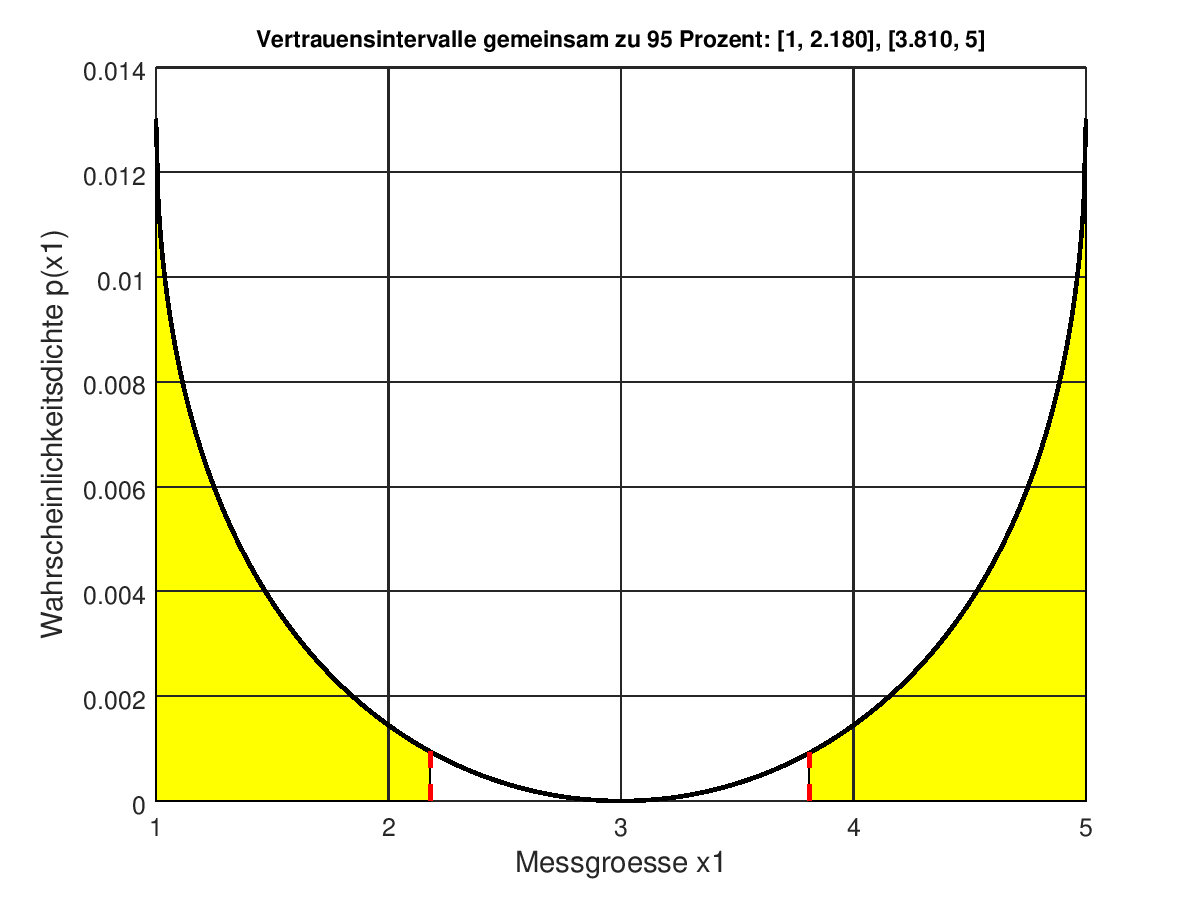
\includegraphics[width=80mm]{10_vorlesung/media/pdf_Uverteilung_Vertrauensniveau.png}
 		\hspace{2mm}
	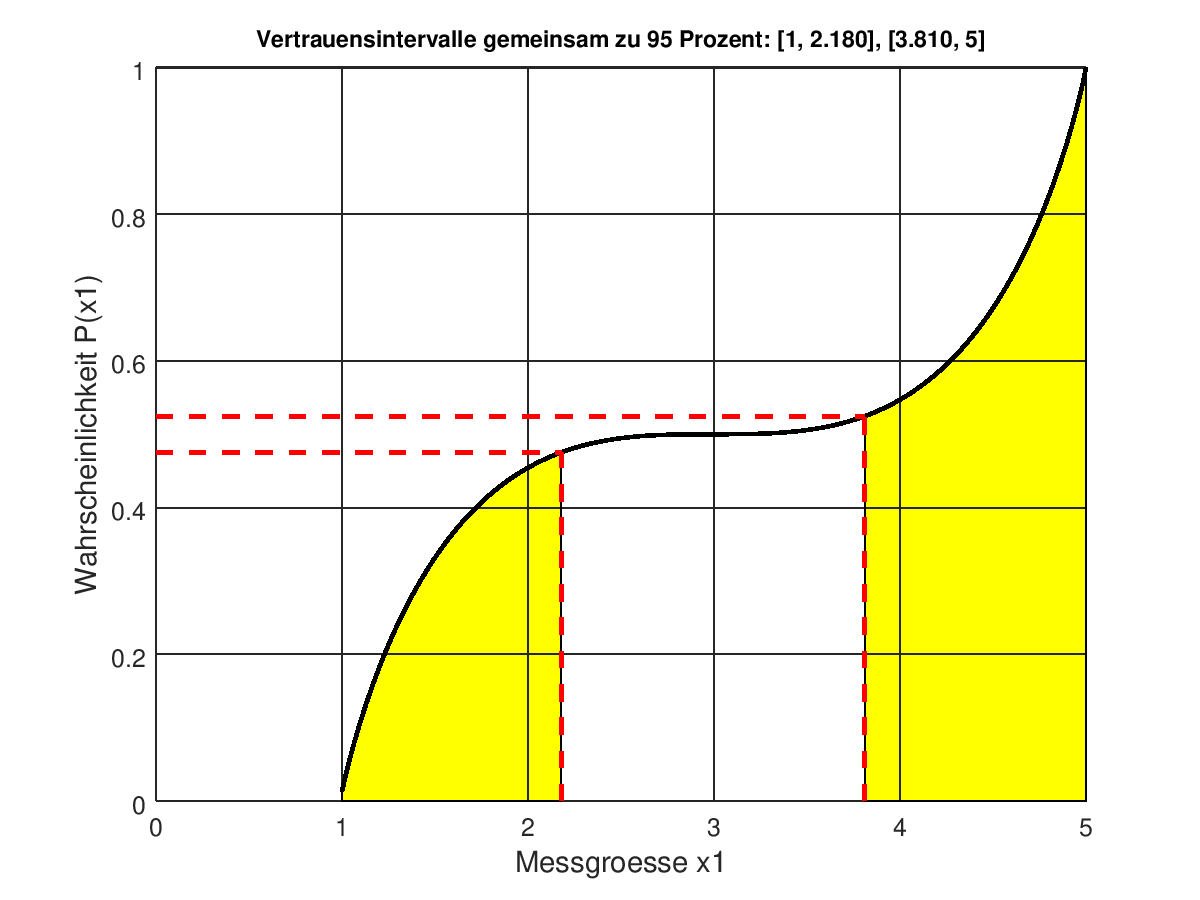
\includegraphics[width=80mm]{10_vorlesung/media/Pkum_Uverteilung_Vertrauensniveau.png}
		\caption{Für das Vertrauensniveau möchte man das häufigste Vorkommen angeben, bei
			bimodaler Verteilung als von jedem der beiden Peaks ausgehen: Bei $95 \%$
			Vertrauensniveau also jeweils $47,5 \%$ für ein Intervall ganz rechts und
			$47,5 \%$ für ein Intervall ganz links, hier als gelbe Flächen markiert.}
		\label{Uverteilungsquantile}
	\end{center}
\end{figure}
In der Mitte, nämlich bei $\bar x$ ist die Wahrscheinlichkeit am geringsten.
Das Signifikanzniveau $\alpha$ liegt folglich in der Mitte und nicht am Rand.
Vom $95 \%$ Vertrauensniveau wird jeweils die Hälfte auf jeden der beiden
Peaks am Rand aufgeteilt, also $47.5 \%$ der Fläche der 
Wahrscheinlichkeitsdichtekurve auf den einen Peak und die anderen $47.5 \%$ der Fläche auf den anderen
Peak. Dann müssen wir zwei Intervalle angeben und sagen: Mit $95 \%$ Wahrscheinlichkeit sind
Werte entweder in dem einen oder dem anderen Intervall zu erwarten, siehe Abb.~\ref{Uverteilungsquantile}.

Die Rechteckverteilung liefert für jeden Wert der Größe $X$ dieselbe Wahrscheinlichkeit für
das liegen innerhalb einer Spanne und die Wahrscheinlichkeit Null außerhalb.
Wenn $s$ die halbe Spanne ist, dann ist die rechteckverteilte Wahrscheinlichkeitsdichteverteilung
\begin{equation}
p(X) \; = \; \left\{\begin{array}{lll}
\frac{1}{2 s} & \text{für} & \bar x - s  \leq X \leq \bar x + s\\
0 & \text{für} &  (X < \bar x - s) \vee (\bar x + s < X)
\end{array}\right. .
\label{rechteckvert}
\end{equation}
Hier kann man nicht entscheiden, wo der Bereich des Signifkanzniveaus und wo der des
Vertrauensniveaus hinzulegen ist.

\subsection{Wahrscheinlichkeitsdichten im Fortpflanzungsgesetz}
Wir betrachten ein einfaches Beispiel eines linearen Modells, bei dem eine
indirekte Messgröße $Y$ von zwei direkten Messgrößen $X_1$ und $X_2$ linear abhängt, also
\begin{equation}
Y = a X_1 + b X_2
\end{equation}
wobei $a$ und $b$ Konstanten sind. Diese Konstanten sind für das Fortpflanzungsgesetz
dann auch direkt die Sensitivitäten: $c_1 = a$ und $c_2 = b$.

Bei diesem Beispiel soll $X_1$ eine Größe darstellen, die nicht der Voraussetzung genügt, gauß- oder
t-verteilt zu sein. Wir untersuchen zwei Fälle, einerseits den Fall, dass sie U-verteilt mit
der Amplitude $s_1$ sei, also $p(X_1)$ gemäß Gl.~(\ref{uverteilung}), andererseits den Fall, 
dass sie rechteckverteilt sei, $p(X_1)$ gemäß Gl.~(\ref{rechteckvert}), mit der halben Spanne $s_1$.

Die Größe $X_2$ sei gaußverteilt.

Konkret verwenden wir hier beispielhaft folgende Zahlenwerte:
\begin{center}
	\begin{tabular}{c|c||c|c||c|c}
		$c_1 = a$ & $c_2 = b$ & $\bar x_1$ & $s_1$ & $\bar x_2$ & $s_2$ \\
		\hline
		$1$ & $1$ & $3$ & $2$ & $3.5$ & $0.5$
	\end{tabular}
\end{center}

Die Wahrscheinlichkeitsdichteverteilung als Funktion der beiden direkten Größen $X_1$
und $X_2$ ist in Abb.~\ref{pdfx1x2} dargestellt, für die U-Verteilung von $X_1$ links
und für die Rechteckverteilung von $X_1$ rechts:
\begin{equation}
p(X_1, X_2) \; = \; p(X_1) \; \underbrace{\frac{1}{\sqrt{2\pi} s_2} 
	e^{-\frac{1}{2}\left(\frac{X_2 - \bar x_2}{s_2}\right)^2} }_{p(X_2)}.
\end{equation}
\begin{figure}
	\begin{center}
		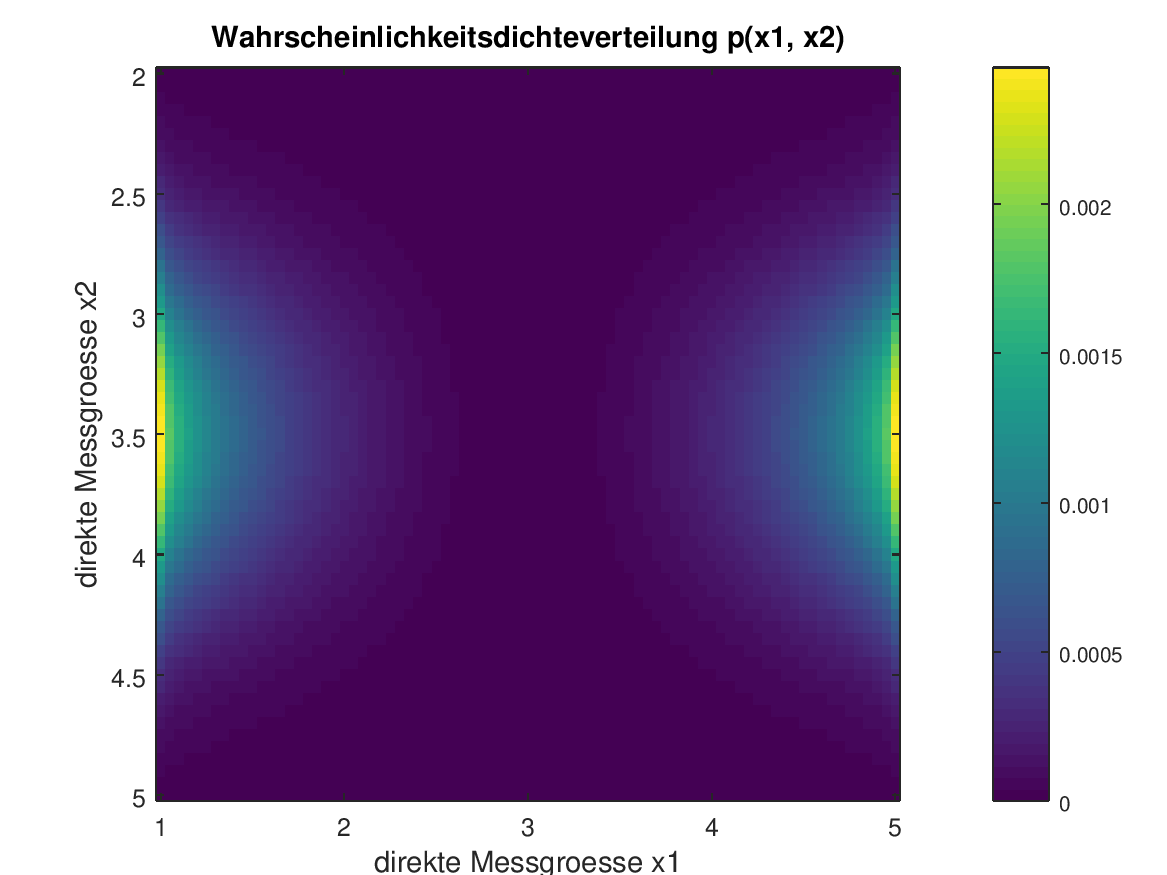
\includegraphics[width=80mm]{10_vorlesung/media/direkte_x1_x2.png}
		\hspace{2mm}
		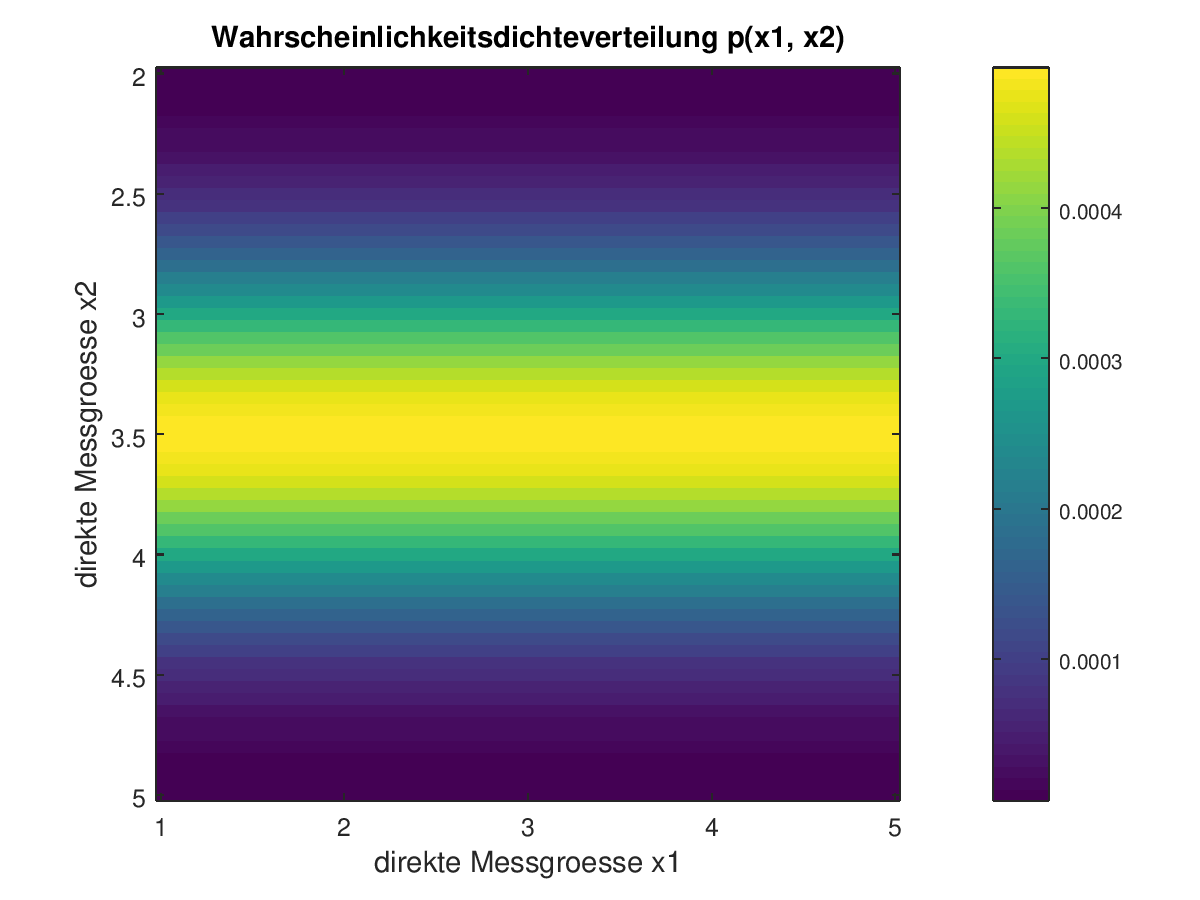
\includegraphics[width=80mm]{10_vorlesung/media/direkte_x1_x2_box.png}
		\caption{Die Wahrscheinlichkeitsdichteverteilung als Funktion der beiden direkten Größen $X_1$
			und $X_2$: \textsl{Links:} U-verteilte Größe $X_1$,
			\textsl{rechts:} rechteckverteilte Größe $X_1$.}
		\label{pdfx1x2}
	\end{center}
\end{figure}

Die Wahrscheinlichkeitsdichteverteilung als Funktion der indirekten Größe $Y$ ist
die Marginalverteilung $p(Y)$ der Verteilung $p(Y,X_1,X_2)$, die sich aus folgendem Produkt ergibt:
\begin{equation}
p(Y,X_1,X_2) \; = \; C_\mathrm{norm} 
\frac{1}{\sqrt{2\pi} \sigma} e^{-\frac{1}{2}\left(\frac{Y - f(X_1, X_2)}{\sigma}\right)^2}
\, p(X_1,X_2) 
\end{equation}
mit $f(X_1, X_2) = a X_1 + b X_2$ und $\sigma$ für die Unsicherheit des Modells, sowie des
Systems, das die Messvorgänge der direkten Größen verknüpft. Letzendlich steckt dahinter
die Vorstellung, dass die indirekte Größe $Y$ ihrerseits auch eine Zufallsgröße ist, nicht nur
die direkten. Die Konstante $C_\mathrm{norm}$ ist so definiert, dass 
$\iiint p(Y,X_1,X_2) \mathrm{d}X_1 \mathrm{d}X_2 \mathrm{d}Y = 1$ (Normierungsbedingung) erfüllt wird, also
\begin{equation}
C_\mathrm{norm} \; = \; \frac{1}{\int\limits_{-\infty}^{\infty} \int\limits_{-\infty}^{\infty}
	\int\limits_{-\infty}^{\infty} p(Y,X_1,X_2) \mathrm{d}X_1 \mathrm{d}X_2 \mathrm{d}Y } .
\end{equation}

\begin{figure}
	\begin{center}
	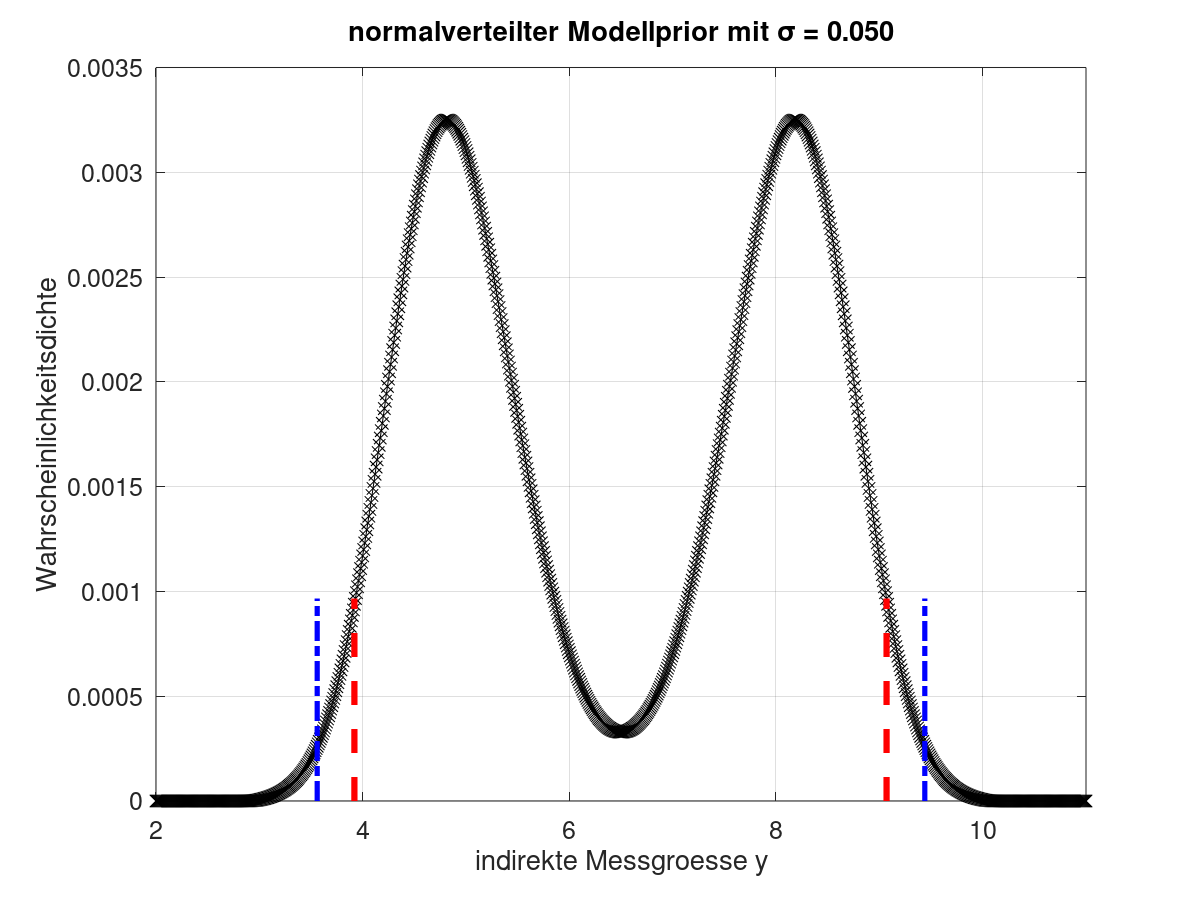
\includegraphics[width=80mm]{10_vorlesung/media/indirekte_y_modellGauss_sigma0p050.png}
		\hspace{2mm}
	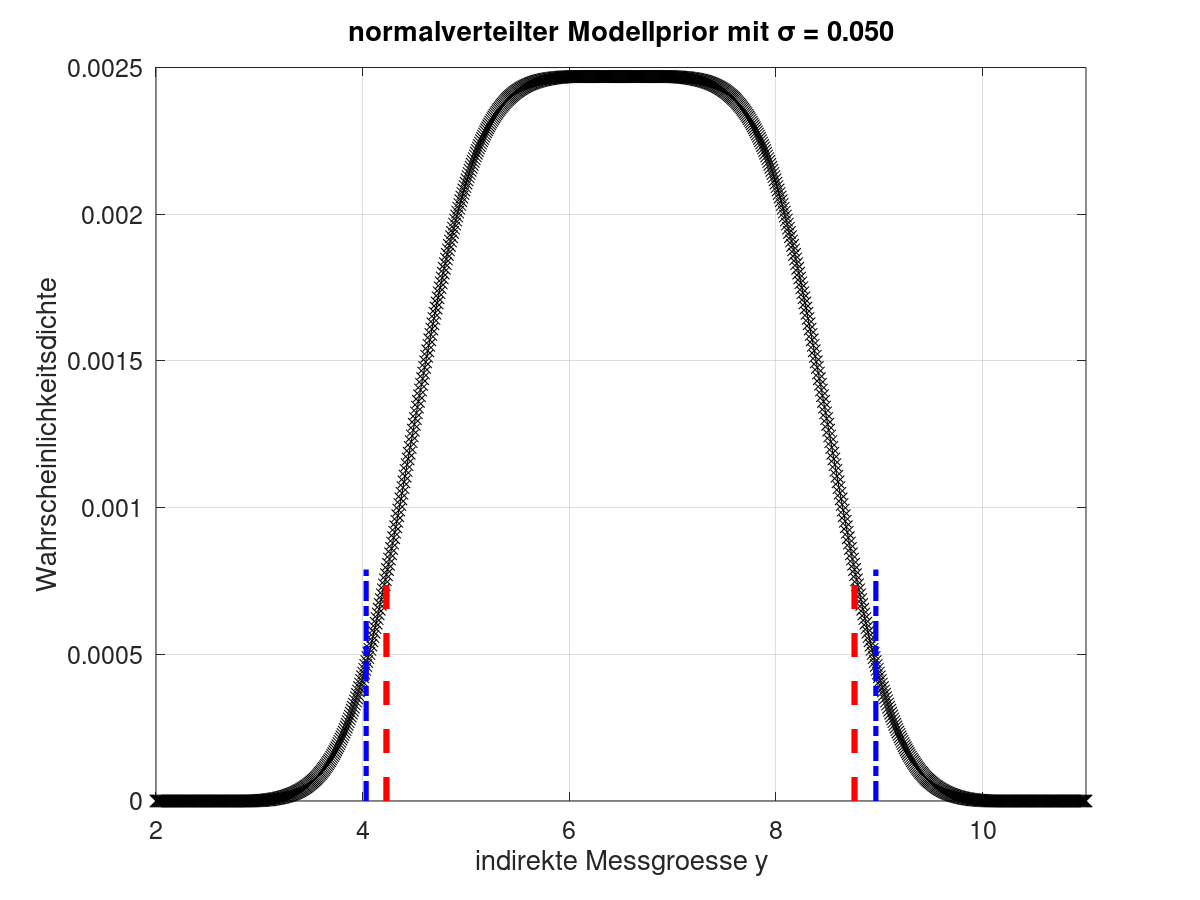
\includegraphics[width=80mm]{10_vorlesung/media/indirekte_y_modellGauss_sigma0p050_box.png}
		\caption{Die Wahrscheinlichkeitsdichteverteilung $p(Y)$ gemäß Gl.~(\ref{pYmarginal}) als Funktion der
			indirekten Größe $Y$ mit Unsicherheit $\sigma = 0.05$ für die Größe $Y$:
			\textsl{Links:} U-verteilte Größe $X_1$,
			\textsl{rechts:} rechteckverteilte Größe $X_1$.}
		\label{pdfYsigma}
	\end{center}
\end{figure}

Für die Vorstellung von einer indirekten Messgröße, die einen exakten wahren Wert haben muss und
die für sich genommen keine Zufallsgröße ist, deren Streuung einzig durch die Streuung der direkten
Größen verursacht wird, wird in der Messtechnik (nirgends sonst in der Statistik) ein
Modellprior verwendet, der durch einen unendlich scharfen Peak repräsentiert wird. 
Wir bezeichnen den (siehe oben) als \textsl{scharfen Modellprior}.

\begin{figure}
	\begin{center}
		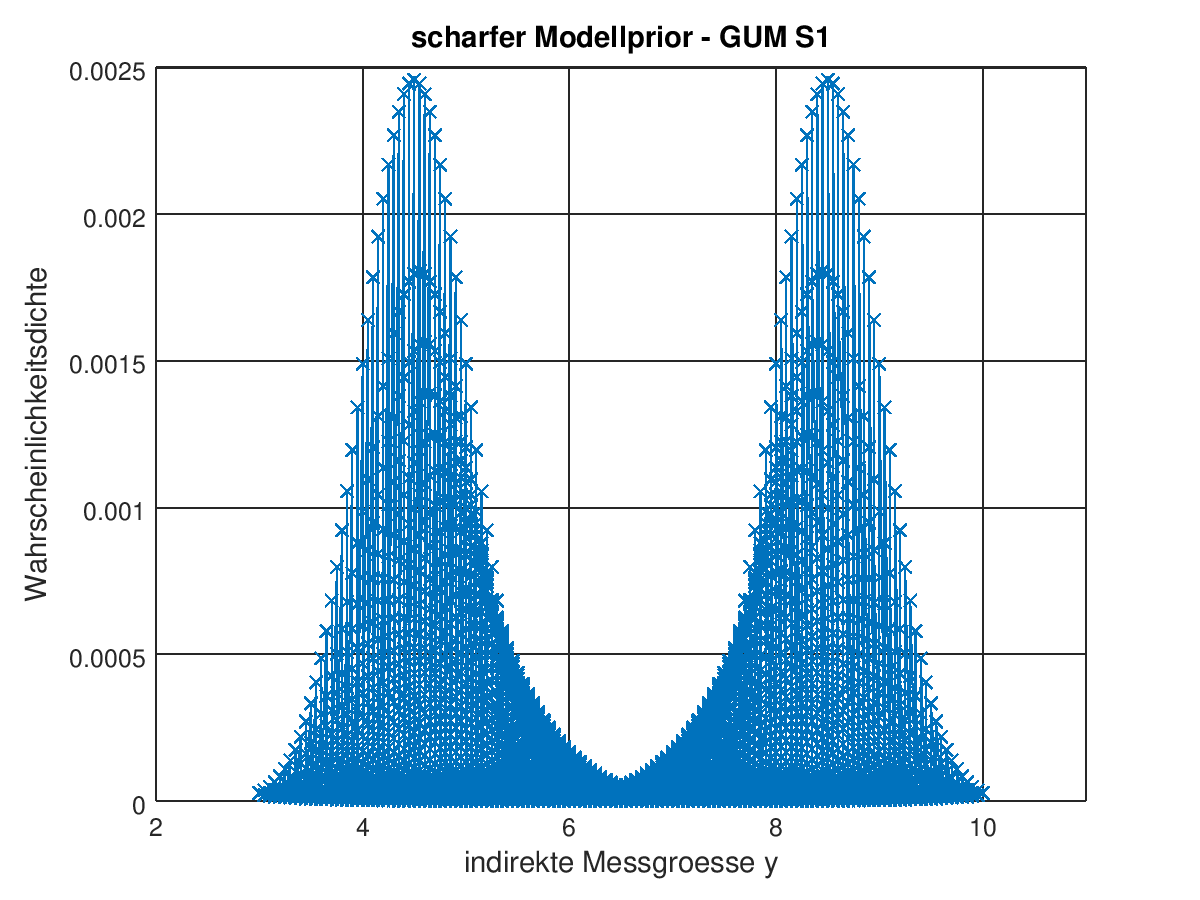
\includegraphics[width=80mm]{10_vorlesung/media/indirekte_ysorted_GUMS1.png}
		\hspace{2mm}
		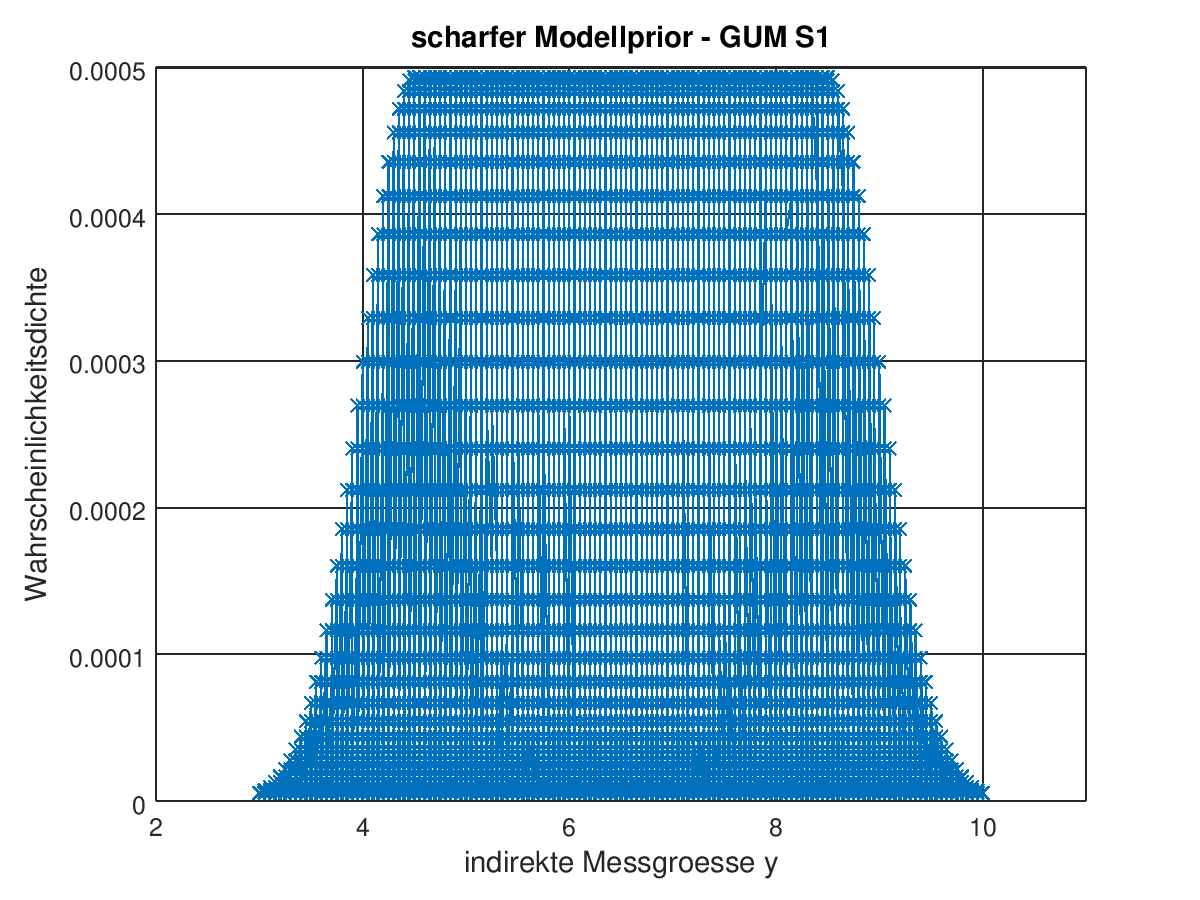
\includegraphics[width=80mm]{10_vorlesung/media/indirekte_ysorted_GUMS1_box.png}
		\caption{Die Wahrscheinlichkeitsdichteverteilung $p(Y)$ gemäß Gl.~(\ref{pYmarginal}) als Funktion der
			indirekten Größe $Y$ mit scharfem Modellprior:
			\textsl{Links:} U-verteilte Größe $X_1$,
			\textsl{rechts:} rechteckverteilte Größe $X_1$.}
		\label{pdfYscharf}
	\end{center}
\end{figure}

Für den scharfen Modellprior für das Verfahren in GUM-Supplement 1 machen wir den Grenzübergang
\begin{equation}
\lim_{\sigma \rightarrow 0} \left\{
\frac{1}{\sqrt{2\pi} \sigma} e^{-\frac{1}{2}\left(\frac{Y - f(X_1, X_2)}{\sigma}\right)^2}
\right\} \; = \; \delta(Y - f(X_1, X_2))
\end{equation}
wobei $\delta$ die dirac'sche Deltadistribution ist.

Die Marginalverteilung $p(Y)$, die die Wahrscheinlichkeitsdichte der indirekten Größe darstellt, ist
\begin{equation}
p(Y) \; = \;  \int\limits_{-\infty}^{\infty}
\int\limits_{-\infty}^{\infty} p(Y,X_1,X_2) \mathrm{d}X_1 \mathrm{d}X_2 .
\label{pYmarginal}
\end{equation}
Sie ist in Abb.~\ref{pdfYsigma} für einen gaußglockenförmigen Modellprior mit $\sigma = 0.05$ und in
Abb.~\ref{pdfYscharf} für einen scharfen Modellprior dargestellt.

In den beiden Abbn.~\ref{pdfYsigma} und \ref{pdfYscharf} auf der linken Seite gezeigten
Diagrammen ist die Marginalverteilung für $Y$ für den Fall dargestellt, dass die direkte Größe 
$X_1$ U-verteilt ist. Sie weist zwei Peaks auf, d.h.\ sie ist bimodal.
Hier müsste man sich also genau anschauen, wo das Signifikanzniveau anzusiedeln ist, also, ob ein
Teil davon in den mittleren Bereich gehört. Der Fall mit rechteckverteilter Größe $X_1$ ist
in dieser Hinsicht gutmütig, so dass wir hier wie gewohnt von der Umkehrfunktion $P^{-1}$ der kumulativen
Verteilung $P(Y)$ die entsprechenden Werte $P^{-1}(\alpha/2)$ und $P^{-1}(1-\alpha/2)$ für
das Vertrauens- oder Überdeckungsintervall nehmen können,
siehe Abb.~\ref{PkumY}.
\begin{figure}
	\begin{center}
	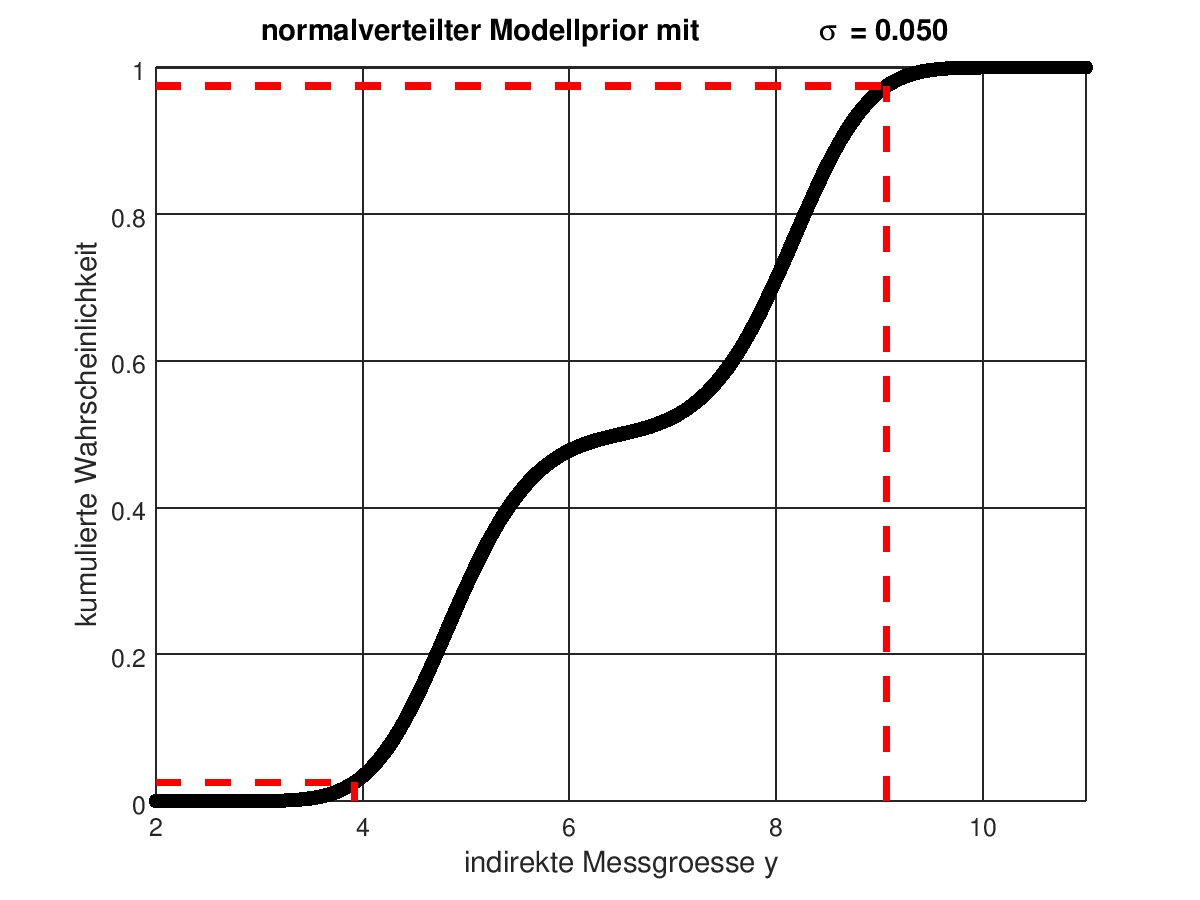
\includegraphics[width=80mm]{10_vorlesung/media/Pkum_indirekte_y_Gauss_sigma0p050.png}
		\hspace{2mm}
	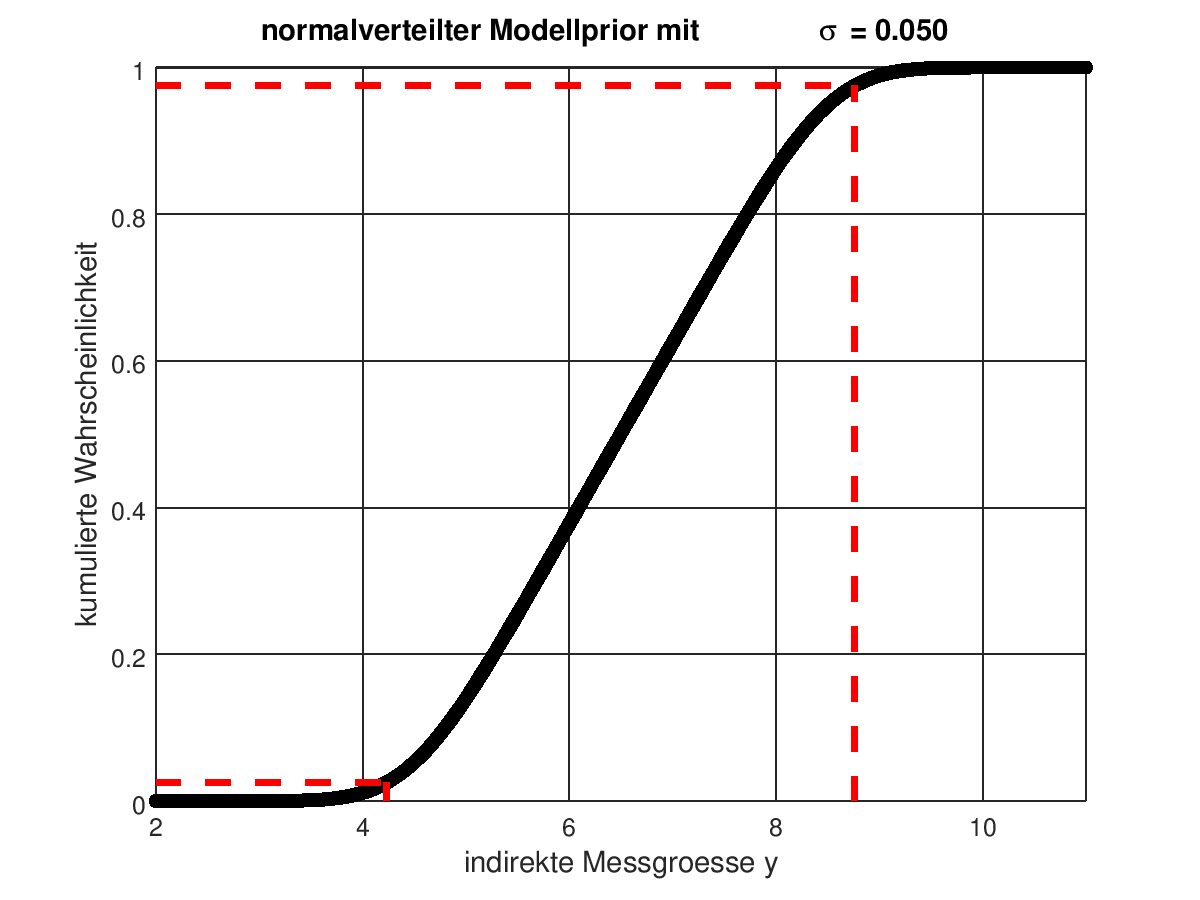
\includegraphics[width=80mm]{10_vorlesung/media/Pkum_indirekte_y_Gauss_sigma0p050_box.png}
		\caption{Die zur kumulierten Verteilung $P(Y)$ der Wahrscheinlichkeitsdichteverteilung $p(Y)$ 
			erworbene Umkehrfunktion liefert mit $P^{-1}(\alpha/2)$ und $P^{-1}(1-\alpha/2)$ zum
			Signifikanzniveau $\alpha$ das entsprechende Vertrauensintervall:
			\textsl{Links:} U-verteilte Größe $X_1$,
			\textsl{rechts:} rechteckverteilte Größe $X_1$.}
		\label{PkumY}
	\end{center}
\end{figure}
Diese Vorgehensweise übernehmen wir hier einfach auch für das Beispiel mit der U-Verteilung. Die in den Diagrammen in Abb.~\ref{pdfYsigma} gestrichelt rot
eingezeichneten Linien kennzeichnen die Vertrauensintervalle.

Zum Vergleich sind in diesen Abb.~\ref{pdfYsigma} die Überdeckungsintervalle, die 
man aus dem Fortpflanzungsgesetz des GUM von 1995/2008 erhalten würde mit blauer
Strichpunktlinie eingezeichnet. Gemäß dem GUM soll für U-verteilte
Größen der Ansatz für die Unsicherheit $u = \mathrm{Spanne}/\sqrt{8}$ und für 
rechteckverteilte
$u = \mathrm{Spanne}/\sqrt{12}$ verwendet werden. Mit $s_1$ als halbe Spanne ist dies
also
\begin{equation}
u^2(X_1) \, = \, \frac{(2 s_1)^2}{8} \, = \, \frac{s_1^2}{2} \quad \text{bzw.}
\quad u^2(X_1) \, = \, \frac{(2 s_1)^2}{12} \, = \, \frac{s_1^2}{3}
\end{equation}
so dass
\begin{equation}
\renewcommand{\arraystretch}{1.3}
u^2(Y) \; = \; \left\{\begin{array}{ll}
a^2 \, \frac{s_1^2}{2} \; + \; b^2 \, s_2^2 & \text{für U-verteilte~} X_1\\
a^2 \, \frac{s_1^2}{3} \; + \; b^2 \, s_2^2 & \text{für rechteckverteilte~} X_1
\end{array}\right. .
\label{GUMMUFF}
\end{equation}
Das Vertrauensintervall, durch die blaue Strichpunktlinie gekennzeichnet, ergeben sich mit den Quantile der Gaußverteilung $z_{\alpha/2} = -1.96$ und $z_{1-\alpha/2} = 1.96$ zu: 
\begin{equation}
[\bar y \; - \; 1.96 \, u(Y), \; \bar y \; + \; 1.96 \, u(Y)]
\; = \; \left\{\begin{array}{ll}
[3.56, 9.44] & \text{für U-verteilte~} X_1\\
\left[4.03, 8.97\right] & \text{für rechteckverteilte~} X_1\\
\end{array}\right.
\end{equation}
mit $\bar y = a \bar x_1 + b \bar x_2$.

Die Werte aus der Marginalverteilung $p(Y)$ im Vergleich dazu sind
\begin{equation}
[P^{-1}(\alpha/2), \; P^{-1}(1 - \alpha/2)]
\; = \; \left\{\begin{array}{ll}
[3.92, 9.07] & \text{für U-verteilte~} X_1\\
\left[4.23, 8.76\right] & \text{für rechteckverteilte~} X_1\\
\end{array}\right.
\end{equation}
für die Breite der Verteilung des Modellprior $\sigma = 0.05$. Sie bilden das
Überdeckungsintervall, das mit roten gestrichelten Linien eingezeichnet ist. Es ist kleiner als das gemäß GUM, Gl~(\ref{GUMMUFF}), ermittelte und zeigt sehr schön, dass
U-verteilte und rechteckverteilte Messgrößen bei der Behandlung mit dem klassischen
Fehlerforpflanzungsgesetz zu falschen Vertrauensintervallen führen kann. 
 
Der dazugehörige Octavecode lautet:
\begin{verbatim}
function non_belldistri_linmodel (sigma=0.05)
% sigma = 0.05, d.h. der Modellparanmter y wird hier mit gaussfoermigem 
% Modellprior, aber sehr schmal, fast dirac'sche delta-Distribution angenommen.

close all

% Falls das Statistikpaket noch nicht geladen ist, kann es wie folgt geladen werden:
% Entsprechend die folgende Zeile ein- oder auskommentieren
pkg load statistics

boxflag = 0; % 0: U-Verteilung; 1: Rechteck-Verteilung;

pltflag1 = 1;
pltflag1a = 0;
pltflag2 = 1;
pltflag3 = 1;

a = 1.0;
b = 1.0;
x1_quer = 3.0;
% Spanne
s1 = 2.0;
%
x2_quer = 3.5;
% Standardabweichung
s2 = 0.5;
%
% Modellgleichung y = a x1 + b x2
%
% Zeilenvektor
x1 = [-s1:0.05:s1] + x1_quer;
if boxflag
p1 = ones(size(x1));
else
p1 = asin((x1 - x1_quer)/s1).^2;
end
p1 = p1/sum(p1);
figure(1);
plot(x1, p1, 'k-');
grid on;
xlabel('direkte Messgroesse x1', 'fontsize', 14);
ylabel('Wahrscheinlichkeitsdichte p(x1)', 'fontsize', 14);
set(gca, 'fontsize', 12);
if pltflag1
print(1,'direkte_x1_box.png', '-dpng');
end
%
% Spaltenvektor
x2 = [-3*s2:0.05:3*s2]' + x2_quer;
p2 = normpdf(x2, x2_quer, s2);
p2chk = exp(-0.5 * ((x2 - x2_quer)/s2).^2) / (sqrt(2*pi) * s2);
figure(2);
plot(x2, p2, 'k-', x2, p2chk, 'r--');
grid on;
xlabel('direkte Messgroesse x2', 'fontsize', 14);
ylabel('Wahrscheinlichkeitsdichte p(x2)', 'fontsize', 14);
set(gca, 'fontsize', 12);
if pltflag2
print(2,'direkte_x2.png', '-dpng');
end
%
% Spalte mal Zeile liefert Matrix
pgesamt = p2*p1;
pgesamt = pgesamt / sum(pgesamt(:));
%
figure(3);
imagesc(x1, x2, pgesamt);
colorbar();
xlabel('direkte Messgroesse x1', 'fontsize', 14);
ylabel('direkte Messgroesse x2', 'fontsize', 14);
title('Wahrscheinlichkeitsdichteverteilung p(x1, x2)', 'fontsize', 14);
set(gca, 'fontsize', 12);
if pltflag1
print(3,'direkte_x1_x2_box.png', '-dpng');
end
%
% ----
%  x1 und x2 in Matrizen fuellen
n2_r = length(x2)
n1_c = length(x1)
X_1 = ones(n2_r,1) * x1;
X_2 = x2 * ones(1, n1_c);
Y_matrix = a*X_1 + b*X_2;
%
% nun als 1D arrays
y = Y_matrix(:);
p_y = pgesamt(:);
figure(4);
plot(y, p_y);
axis([2 11]);
title('scharfer Modellprior - GUM S1', 'fontsize', 14);
xlabel('indirekte Messgroesse y', 'fontsize', 14);
ylabel('Wahrscheinlichkeitsdichte', 'fontsize', 14);
set(gca, 'fontsize', 12);
if pltflag1a
print(4,'indirekte_y_GUMS1.png', '-dpng');
end
%
% sortieren, so dass y monoton steigend ist
[ys, isort] = sort(y);
p_sort = p_y(isort);
figure(5);
plot(ys, p_sort, 'x-');
axis([2 11]);
grid on;
title('scharfer Modellprior - GUM S1', 'fontsize', 14);
xlabel('indirekte Messgroesse y', 'fontsize', 14);
ylabel('Wahrscheinlichkeitsdichte', 'fontsize', 14);
set(gca, 'fontsize', 12);
if pltflag1
print(5,'indirekte_ysorted_GUMS1_box.png', '-dpng');
end

%
% mit gaussfoermigem Modellprior, aber sehr schmal, fast dirac'sche delta-Distribution
%
dy = 0.01;
y_model = [2:dy:11];
n_model = length(y_model);
%  sigma = 0.5;
p_mod = zeros(1, n_model);
for k = 1:n_model
%
% Summationen entsprechen der Integration ueber x1 und x2
% zum Berechnen der Marginalverteilung
p_mod(k) = sum(sum(exp(-0.5 * ((y_model(k) - Y_matrix)/sigma).^2) .* pgesamt));
end
Pkum = cumsum(p_mod);
psum = Pkum(n_model);
Pkum = Pkum/psum;
p_mod = p_mod/psum;

%
% Signifikanzniveau
alpha = 0.05;
%
% Quantile
[left, ileft] = min(abs(Pkum - alpha/2))
[right, iright] = min(abs(Pkum - (1-alpha/2)))
%
erw_y = sum(y_model .* p_mod);
std_y = sqrt(sum((y_model - erw_y).^2 .* p_mod));
%
% Vergleich mit Fortpflanzungsgesetz, das eigentlich nur fuer
% glockenfoermige Verteilungen gilt, bei denen die Wurzel des zweiten statistischen
% Moments, also die Varianz die Breite der Verteilung definiert, bzgl der sie
% sich normieren laesst.
y_quer = a*x1_quer + b*x2_quer;
if boxflag
u_y = sqrt((a * s1)^2/3 + (b * s2)^2);
else
u_y = sqrt((a * s1)^2/2 + (b * s2)^2);
end
%
figure(6);
sigma_str = num2str(sigma,'%1.3f');
plot(y_model, p_mod, 'kx-', ...
[y_quer-1.96*u_y, y_quer-1.96*u_y], [0, p_mod(iright)], 'b-.', 'linewidth', 2.5, ...
[y_quer+1.96*u_y, y_quer+1.96*u_y], [0, p_mod(iright)], 'b-.', 'linewidth', 2.5, ...
[y_model(ileft), y_model(ileft)], [0, p_mod(iright)], 'r--', 'linewidth', 3, ...
[y_model(iright), y_model(iright)], [0, p_mod(iright)], 'r--', 'linewidth', 3);
% plot(y_model, p_mod, 'kx-', ...
%  [y_quer-1.96*u_y, y_quer-1.96*u_y], [0, p_mod(iright)], 'b-.', 'linewidth', 2.5, ...
%  [y_quer+1.96*u_y, y_quer+1.96*u_y], [0, p_mod(iright)], 'b-.', 'linewidth', 2.5, ...
%  [erw_y-1.96*std_y, erw_y-1.96*std_y], [0, p_mod(iright)], 'g-', 'linewidth', 2.5, ...
%  [erw_y+1.96*std_y, erw_y+1.96*std_y], [0, p_mod(iright)], 'g-', 'linewidth', 2.5, ...
%  [y_model(ileft), y_model(ileft)], [0, p_mod(iright)], 'r--', 'linewidth', 3, ...
%  [y_model(iright), y_model(iright)], [0, p_mod(iright)], 'r--', 'linewidth', 3);
grid on;
axis([2 11]);
title(['normalverteilter Modellprior mit \sigma = ', sigma_str], 'fontsize', 14);
xlabel('indirekte Messgroesse y', 'fontsize', 14);
ylabel('Wahrscheinlichkeitsdichte', 'fontsize', 14);
set(gca, 'fontsize', 12);
if pltflag3
print(6,['indirekte_y_modellGauss_sigma', strrep(sigma_str,'.','p'),'_box.png'], '-dpng');
end

%
figure(7);
plot(y_model, Pkum, 'ko-', ...
[y_model(ileft), y_model(ileft)], [0, Pkum(ileft)], 'r--', 'linewidth', 3, ...
[y_model(iright), y_model(iright)], [0, Pkum(iright)], 'r--', 'linewidth', 3, ...
[y_model(1), y_model(ileft)], [Pkum(ileft), Pkum(ileft)], 'r--', 'linewidth', 3, ...
[y_model(1), y_model(iright)], [Pkum(iright), Pkum(iright)], 'r--', 'linewidth', 3);
grid on;
axis([2 11]);
title(['normalverteilter Modellprior mit \sigma = ', sigma_str], 'fontsize', 14);
xlabel('indirekte Messgroesse y', 'fontsize', 14);
ylabel('kumulierte Wahrscheinlichkeit', 'fontsize', 14);
set(gca, 'fontsize', 12);
if pltflag3
print(7,['Pkum_indirekte_y_Gauss_sigma', strrep(sigma_str,'.','p'),'_box.png'], '-dpng');
end
%
printf('Modellprior mit sigma = %1.3f\n', sigma);
printf('Erwartungswerte:\n');
printf('aus Erw von x1 und x2:  %1.2f\n', y_quer);
printf('aus Verteilung p_model: %1.2f\n', erw_y);
printf('Standardabweichungen als Wurzel der Varianz:\n');
printf('aus Fortpflanzung klassisch: %1.2f\n', u_y);
printf('aus Verteilung p_model:      %1.2f\n', std_y);
printf('Ueberdeckungsintervall fuer 95 Prozent\n');
printf('aus Fortpflanzung klassisch mit Quantil aus Gaussvert 1.96:  [%1.2f, %1.2f]\n',
y_quer - 1.96*u_y, y_quer + 1.96*u_y);
printf('aus Verteilung p_model, ueber die Umkehrfkt der kumulativen: [%1.2f, %1.2f]\n',
y_model(ileft), y_model(iright));
end
\end{verbatim}

\begin{thebibliography}{------}
    \bibitem[Els07]{Els07} C. Elster: Calculation of unceratinty
	in the presence of prior knowledge, Metrologia 44, 111-116, (2007)
    \bibitem[Cox06]{Cox06} M.G. Cox, B.R.L. Siebert:The use of
    a Monte Carlo method for evaluating ..., Metrologie 43, S178-88,
    (2006)
    \bibitem[GUMS1]{GUMS1} 
    JCGM 101:2008; Evaluation of measurement data — Supplement 1 to the 
    “Guide to the expression of uncertainty in measurement” — 
    Propagation of distributions using a Monte Carlo method (2008); \newline 
    https://www.bipm.org/utils/common/documents/jcgm/JCGM\_101\_2008\_E.pdf
    \bibitem[Wue08]{Wue08} Gerd Wübbeler, Michael Krystek and Clemens Elster: Evaluation of measurement uncertainty
    and its numerical calculation by a Monte Carlo method
    Meas. Sci. Technol. 19 (2008) 084009 (4pp)
    doi:10.1088/0957-0233/19/8/084009
    \end{thebibliography}

\newpage
\section{Anhang}
\subsection{A1: Matlab-Skript zum Delta-Peaken mit Bayes}
\lstinputlisting[style=Matlab]{10_vorlesung/code/bayes_indirect_quantity.m}
\subsection{A2: Octave-Skript zur Fehlerfortpflanzung mit U- und Rechteck-Verteilungen}
\lstinputlisting[style=Matlab]{10_vorlesung/code/non_belldistri_linmodel.m}

\begin{comment}
\begin{verbatim}
function bayes_indirect_quantity()
% Hueser, 17-11-25
close all, clear all
%	Kalibrierfaktor
K_faktor_0 = 0.0925;
sigma_K = 0.0090;
%	Unsicherheit Messgeraet
sigma_M = 0.3; % Volt
%
%
JM = 11;
sig = 12;
mue = 500;
data_M = mue + sig*randn( JM,1);
%
%
xK = [-4*sigma_K:0.001:4*sigma_K] + K_faktor_0;
nK = length(xK)
xM = [-4*sig:0.1:4*sig] + mue;
nM = length(xM)
y = [20:0.2:80];
nY = length(y)
%
std_M = std(data_M)*1.7;
std_KM = K_faktor_0 * std_M;
%
% Messungen in Volt
XM = data_M * ones(1,nM) - ones(JM,1) * xM;
%
% Das Modell: y = f(xK, xM)
% für jedes xK und jedes xM kombiniert
% y_{KM,i,j} = xK_i * xM_j für alle i=1,..,nK und j=1,..,nM
y_KM_matrix = xK' * xM;
%  in einen langen Spaltenvektor gebracht
y_KM = y_KM_matrix(:);
nKM = length(y_KM);
delta_y = y_KM * ones(1,nY) - ones(nKM, 1)*y;

% direkte Groessen
% Kalibrierfaktor
p_K = exp(-0.5 * ( (xK - K_faktor_0)/sigma_K ).^2 );
p_K = p_K / sum(p_K);
figure(110);
plot( xK, p_K,'linewidth',2);
xlabel('Kalibrierfaktor / (Einheit/Volt)', 'fontsize', 14);
ylabel('pdf', 'fontsize', 14);
set(gca, 'fontsize', 14);

set(gcf, 'PaperUnits', 'centimeters');
x_width=15 ;y_width= 8;
set(gcf, 'PaperPosition', [0 0 x_width y_width]);
print '-dpng' Kalibrierfaktor.png

% Messungen mit der kleinen Streuung
p_M_matrix = exp(-0.5 * ( XM/sigma_M ).^2 );
%   Summe über alle Messungen
p_M_1 = sum( p_M_matrix );
p_M_1 = p_M_1 / sum(p_M_1);
% mit der grossen Streuung
p_M_matrix = exp(-0.5 * ( XM/std_M ).^2 );
%   Summe über alle Messungen
p_M_2 = sum( p_M_matrix );
p_M_2 = p_M_2 / sum(p_M_2);
figure(111);
plot(xM, p_M_1,'k-', ...
xM, p_M_2,'r--','linewidth',2);
xlabel('Rohdaten / Volt', 'fontsize', 14);
ylabel('pdf', 'fontsize', 14);
legend('Geraet genau','Geraet ungenau','fontsize',14)
set(gca, 'fontsize', 14);
set(gcf, 'PaperUnits', 'centimeters');
x_width=15 ;y_width= 8;
set(gcf, 'PaperPosition', [0 0 x_width y_width]);
print '-dpng' Rohdaten.png
%
% PWahrscheinlichkeit als Funktion der beiden
% direkten Groessen xK und xM
p_KM_matrix = p_K' * p_M_1;
%  in einen langen Spaltenvektor gebracht
p_KM_1 = p_KM_matrix(:);
%
p_KM_matrix = p_K' * p_M_2;
%  in einen langen Spaltenvektor gebracht
p_KM_2 = p_KM_matrix(:);


%
% Wahrscheinlichkeitsdichteverteilung des Modells
% zur Vereinfachung nehme ich jetzt keine 
% Verteilung um die std_m sondern nur den einen Schätzwert
p_y = exp(-0.5 * ( delta_y/std_KM ).^2 );
%
%	posterior
post_matrix = p_y .* (p_KM_1 * ones(1,nY));
sumpost = sum(post_matrix(:));
post_matrix = post_matrix/sumpost;
%
% Marginalverteilung durch Summation über xM, xK
posterior1 = sum(post_matrix);
%
%
%	posterior
post_matrix = p_y .* (p_KM_2 * ones(1,nY));
sumpost = sum(post_matrix(:));
post_matrix = post_matrix/sumpost;
%
% Marginalverteilung durch Summation über xM, xK
posterior2 = sum(post_matrix);
%
%
p_y2 = exp(-0.5 * ( delta_y/(std_KM*0.003) ).^2 );
%	posterior
post_matrix = p_y2 .* (p_KM_2 * ones(1,nY));
sumpost = sum(post_matrix(:));
post_matrix = post_matrix/sumpost;
%
% Marginalverteilung durch Summation über xM, xK
posterior3 = sum(post_matrix);

[y_KMsort, km_sort] = sort(y_KM);
p_2 = p_KM_2(km_sort);
diff_y = diff(y_KMsort);
mid_p_KM_2 = (p_2(2:nKM)+p_2(1:nKM-1))*0.5;
iuse = find(diff_y>0);
meandiff = mean(diff_y(iuse))
diff_y = diff_y/meandiff;
pdf = mid_p_KM_2(iuse)./diff_y(iuse);
figure(120);
plot(diff_y);
figure(121);
plot(y_KMsort(iuse),pdf);
sumpdf = 5.2e6; max(pdf)
figure(100);
plot( y_KMsort(iuse), max(posterior1)*pdf/sumpdf, 'g.',...
y, posterior1,'k-',...
y, posterior2,'r--',...
y, posterior3,'b-','linewidth',2);
xlabel('indirekte Groesse / Einheit', 'fontsize', 14);
ylabel('pdf', 'fontsize', 14);
legend('Dirac: Weise/Wuebbler','Geraet genau, Messobj schlecht',...
'beides ungenau','Geraet ungenau, Modell duenner Peak')
% axis([10 100]);
% set(gca, 'fontsize', 14);
set(gcf, 'PaperUnits', 'centimeters');
x_width=15 ;y_width= 8;
set(gcf, 'PaperPosition', [0 0 x_width y_width]);
print '-dpng' Posterior_all.png
\end{verbatim}
\end{comment}
\newpage
\section{Übungsaufgaben}
\textbf{Aufgabe 10-1: Bestimmung des Schätzwertes und der Messunsicherheit bei
einem linearen Modell und Normalverteilungen}\\
Gegeben ist ein linearer Zusammenhang zwischen der Ausgangsgröße (indirekte
Messgröße) $Y$ und den Eingangsgrößen $X_j$ (direkte Messgrößen) wie folgt:
\[
Y = c_1 \cdot X_1 + c_2 \cdot X_2
\]
Die direkten Messgrößen $X_1$ und $X_2$ sind nicht korreliert und 
normalverteilt mit: 
\[
X_1 \sim N_{1}(\mu_1 =x_1=3,\sigma_1^2= 0.5^2 ) 
\quad X_2 \sim N_{2}(\mu_2=x_2= 5,\sigma_2^2=0.2^2 )
\]
Nehmen Sie für $c_1 = 2$ und für $c_2 = 3$ an. 

Als Priorinformation ist bekannt, dass die indirekte Messgröße
normalverteilt ist mit \newline  $N_0(y_0=20,\sigma_0^2=3)$

Bestimmen Sie den Schätzwert $y$ und die dazugehörige Unsicherheit 
$u(y)$ mit den Gl.(\ref{eq:Erwartungswert_y_Normalverteilung}) und 
(\ref{eq:Unsicherheit_y_Normalverteilung})

\textbf{Lösung zu 10-1} \\
Die Kovarianzmatrix ist gegegen durch 
\begin{align}
\boldsymbol{V(X)} &= 
\begin{pmatrix}
\operatorname{Var}(X_1) & 0 \\
0 & \operatorname{Var}(X_2)  \\
\end{pmatrix}
= 
\begin{pmatrix}
\sigma_1^2 & 0 \\
0 & \sigma_2^2 \\
\end{pmatrix}
\end{align}
Für die Unsicherheit von $y$ erhält man mit Vorwissen nach Gl.	(\ref{eq:Unsicherheit_y_Normalverteilung}):
\[
u^2(y) = \left[ \frac{1}{c_1^2\cdot \sigma_1^2 + c_2^2\cdot \sigma_2^2} 
+ \frac{1}{\sigma_0^2} \right]^{-1}
 = \left[ \frac{1}{2^2\cdot 0.5^2 + 3^2\cdot 0.2^2} 
+ \frac{1}{3^2} \right]^{-1} = 1.1815
\]

Für den Schätzwert $y$ ergibt sich nach Gl.(\ref{eq:Erwartungswert_y_Normalverteilung}):
\[
y = u^2(y) \;\left[ \frac{\T c_1\cdot x_1 + c_2\cdot x_2}
{\T c_1^2 \cdot \sigma_1^2 + c_2^2\cdot \sigma_2^2} +\frac{y_0}{\sigma_0^2} \right]
 = 1.1815 \cdot \; \left[\frac{2\cdot 3 + 3\cdot 5}
{2^2 \cdot 0.5^2 + 3^2\cdot 0.2^2} + \frac{20}{3^2} \right] = 20.8867
\]
Als \textbf{Schätzwert} erhält man $y=20.89$ und als \textbf{Unsicherheit} $u(y)= 1.09 $


\begin{thebibliography}{------}
	\item[] \hspace*{5em}{\Large\bf zu Kapitel 10:}
\end{thebibliography}